\mainmatter

\chapter{Einleitung}\label{chap:introduction}
\section{Hintergrund und Kontext}
Durch die zunehmende Globalisierung und Digitalisierung wird die Gesellschaft der Gegenwart und Zukunft geprägt. Der Ausbau von Hochgeschwindigkeitsnetze und die globale Corona-Pandemie haben diese Entwicklung noch einmal beschleunigt. Immer mehr Unternehmen erkennen die Potenziale der Digitalisierung und stellen ihre Geschäftsprozesse um. Ganze Wertschöpfungsketten werden auf cloudbasierte Umgebungen umgestellt. Angefangen bei der Kommunikation, über Beschaffung und Produktion bis zum Verkauf der Waren und Dienstleistungen, vergleiche mit \parencite[Seite 21 ff.]{banholzer-2020} und \cite{oswald-2022}. In allen Stufen der Prozesse kommen webbasierte Anwendungen zum Einsatz, um die Kommunikation der Anwender mit den Systemen zu ermöglichen oder Schnittstellen für die Datenübertragung zwischen den verschiedenen Systemen zu gewährleisten. Durch wachsende Anzahl von Web-Anwendungen wächst auch der Druck für die Entwicklungsfirmen, ihre Anwendungen den schnell und oft wechselnden Kundenanforderungen anzupassen.\vspace{0.2cm}

Durch diesen Prozess getrieben, müssen Entwicklungsfirmen in immer kürzeren Release-Zyklen Softwarekomponenten hinzufügen und vorhandene erweitern. Gleichzeitig wachsen aber auch die Anforderungen an Stabilität und Sicherheit der cloudbasierten Anwendungen, sowie der Bedarf an kostengünstigeren IT-Abläufen (Beweis fehlt). Ein weiteres Problem ist der wachsende Fachkräftemangel in der Wirtschaft und die damit verbundenen steigenden Gehälter der Entwickler (Beweis fehlt).\vspace{0.2cm}

Die Verwendung künstlicher Intelligenz bei der Programmierung gewinnt immer mehr an Bedeutung. Eine Technologie die im besonderen Maße an dieser Entwicklung beteiligt ist, sind die Large Language Models. Insbesondere mit der Veröffentlichung vom ChatGPT wurde hier ein regelrechter Hype um die \acrshort{LLM}s ausgelöst. Diese Modelle erlauben eine Softwareentwicklung mit natürlicher Sprache. Tiefe Kenntnisse der verwendeten Programmiersprache sind nicht mehr in dem Maße erforderlich, wie ohne LLMs.\vspace{0.2cm}


\section{Problemstellung}
So groß der Hype um Künstliche Intelligenz auch sein mag, zurzeit kann KI nicht alle Anforderungen selbstständig lösen. Dies sollte auch bei der Verwendung von KI generierten Inhalten und Programmcodes beachtet werden.

\epigraph[
	source={Vattenfall Online},
	etc={ KI für Unternehmen – die Grenzen der KI},
	author and source indent=0.5cm,
	dash=,
	after skip=0.5cm
]{KI denkt nicht, KI trifft keine Entscheidungen. Eine KI antwortet auf eine Eingabe nicht mit der besten Antwort, sondern mit der Wahrscheinlichsten.}

Der Mensch muss die generierten Ergebnisse überprüfen, ehe erstellte Programmcodestücke in vorhandene Programme eingefügt und in Produktionsumgebungen implementiert werden.\vspace{0.3cm}

Viele Entwickler setzen auf Chatbots, wie ChatGPT oder Gemini zur Generierung von Code, wie eine Umfrage von \textit{stackoverflow} vom Mai 2024 zeigt \cite{noauthor_developers_2024}. Gleichzeitig wachsen auch die technischen Schulden bei Softwareprojekten, da diese Modelle nicht für die Entwicklung von Software optimiert sind (Beweis fehlt).\vspace{0.2cm}

%\subsection{Herausforderungen bei der Entwicklung von Webanwendungen}

%\subsection{Potenzial von LLMs in der Webentwicklung}


\section{Zielsetzung und Forschungsfragen}
Diese Arbeit soll eine Auswahl von Modellen evaluieren und dessen Brauchbarkeit für die Softwareentwicklung aufzeigen. Die Modellauswahl wird von der Seite \href{https://evalplus.github.io/leaderboard.html}{EvalPlus Leaderboard} abgeleitet. Hier werden Modelle gewählt, welche erstere Plätze belegen, aber zum Vergleich auch Modelle aus dem Mittelfeld.\vspace{0.2cm}

Des Weiteren soll gezeigt werden, ob die automatisierte Verwendung beider Techniken eine Effizienz und Effektivität des Entwicklungsprozesses gesteigert werden kann.


\section{Aufbau der Arbeit}
Ein paar Worte zum Aufbau dieser Arbeit. Im Kapitel \ref{chap:state_of_research} wird der aktuelle Stand der Forschung vorgestellt und Erkenntnisse anderer Arbeiten diskutiert. Die in dieser Arbeit verwendetet Methoden, werden im Kapitel \ref{chap:methodology} behandelt. Die Implementierung der Test LLMs wird in Kapitel \ref{chap:implementation} besprochen und in Kapitel \ref{chap:evaluation} die Ergebnisse evaluiert. Bevor in Kapitel \ref{chap:conclusion} auf mögliche Folgearbeiten eingegangen wird, gibt es in Kapitel \ref{chap:application_scenarios} Anwendungsszenarien, die zu den Ergebnissen dieser Arbeit geführt haben.


\section{Abgrenzung}
Ausschluss anderer Anwendungsbereiche.

Rechtliche und ethische Überlegungen werden nur am Rande berücksichtigt.

\chapter{Grundlagen}\label{chap:basics}
In diesem Kapitel werden Grundlagen besprochen die eine Relevanz für diese Arbeit haben. Die angesprochenen Bereiche können nur oberflächlich einen kleinen Einstieg in die jeweiligen Teilgebiete geben.\vspace{0.2cm}

Die Forschungsbereiche der großen Sprachmodelle, kurz \acrshort{LLM} [eng. Large Language Model], ist ein Teilgebiet von Deep Learning und der Forschung von der Verarbeitung natürlicher Sprache, kurz \acrshort{NLP} [eng. Natural Language Processing]. Die Grafik \ref{img:classification_of_terms} zeigt die Einordnung der Bereiche.

\begin{figure}[!ht]
	\includegraphics[width=0.8\textwidth]{content/chapter_basics/images/einordnung_bezeichnungen.eps}
	\centering
	\caption{LLMs im Kontext der Forschungsbereiche von KI}
	\label{img:classification_of_terms}
\end{figure}


\section{Künstliche Intelligenz}
Die künstliche Intelligenz hat bereits in viele Unternehmensprozesse Einzug gehalten. Besonders die generative KI, mit ihren großen Sprachmodellen wird in den nächsten Jahren immer weiter in die Unternehmensbereiche vorstoßen und viele Aufgaben übernehmen. Entscheider und Führungspersonal versprechen sich von der Technologie nicht nur effizientere Prozesse, sondern auch Kosteneinsparungen.\vspace{0.2cm}

Eine explizite Definition für \textit{künstliche Intelligenz} ist zurzeit noch nicht einheitlich erfolgt. Geschuldet ist diese Tatsache, dass der Begriff \textit{Intelligenz} nicht eindeutig definiert ist. Somit finden sich viele Versuche eine Definition für künstliche Intelligenz herzuleiten. In dieser Arbeit wird als Definition für die Künstliche Intelligenz, die aus \cite[6 ff.]{definition_ki2019} verwendet.

\epigraph[
	author={Bitkom e.V.},
	text indent=0.5cm,
	after skip=-1.0cm
	]{
	Systeme der künstlichen Intelligenz (KI-Systeme) sind vom Menschen entwickelte Softwaresysteme (und gegebenenfalls auch Hardwaresysteme), die in Bezug auf ein komplexes Ziel auf physischer oder digitaler Ebene handeln, indem sie ihre Umgebung durch Datenerfassung wahrnehmen, die gesammelten strukturierten oder unstrukturierten Daten interpretieren, Schlussfolgerungen daraus ziehen oder die aus diesen Daten abgeleiteten Informationen verarbeiten, und über das bestmögliche Handeln zur Erreichung des vorgegebenen Ziels entscheiden. KI-Systeme können entweder symbolische Regeln verwenden oder ein numerisches Modell erlernen, und sind auch in der Lage, die Auswirkungen ihrer früheren Handlungen auf die Umgebung zu analysieren und ihr Verhalten entsprechend anzupassen.
}

%(\href{https://www.bitkom.org/sites/main/files/file/import/171012-KI-Gipfelpapier-online.pdf}{Wirtschaftliche Bedeutung ...}, 26 ff.).

%Die folgenden Kapitel werden auf die Teilbereiche der künstlichen Intelligenz eingehen, welche für die Entwicklung der großen Sprachmodelle essenziell sind.
Aus dem Forschungsgebiet der künstlichen Intelligenz ist für die großen Sprachmodelle der Bereich des \glqq Deep Learning\grqq \ besonders interessant. Hier findet die Überschneidung mit dem Bereich der NLP statt, welche massiv dazu betrug, dass die großen Sprachmodelle diesen Erfolg erfahren.

\subsection{Maschinelles Lernen}
Als Teilgebiet der künstlichen Intelligenz befasst es sich mit dem Problem wie Maschinen Lernen und Denken können. Wobei hier nicht von selbstständigem Lernen und Denken gesprochen werden kann, sondern lediglich von Imitieren dieser Prozesse. Aber \acrshort{ML} ist sehr wohl in der Lage aus großen Datenmengen komplexe Muster und Funktionen zu erkennen. Für das maschinelle Lernen gibt es mehrere Formen von Lernparadigmen.\vspace{0.2cm}

Beim \textit{überwachten Lernen} sind für die Eingaben der Trainingsdaten dazugehörige Ausgaben, die Labels definiert. Das Ziel ist es eine Funktion zu trainieren um künftige Eingaben korrekt klassifizieren oder vorhersagen zu können. Dieses Lernparadigma wird häufig eingesetzt, wenn es sich um Regressionens- und Klassifizierungsprobleme handelt.\vspace{0.2cm}

Die gelabelten Ausgaben sind beim \textit{unüberwachten Lernen} nicht vorhanden. Hierbei wird beispielsweise durch Clustering oder Dimensionsreduktion versucht Muster und Strukturen zu erkennen. Des Weiteren soll die Methode helfen Anomalien in Daten zuerkennen aber Assoziationen zwischen Datenobjekten zu finden.\vspace{0.2cm}

Das \textit{selbst überwachte Lernen} ermöglicht es Modellen, sich selbst zu überwachen ohne gelabelte Daten. Hierbei lernen die Algorithmen einen Teil der Eingaben von anderen Teilen und generieren automatisch Labels. So werden unüberwachten Problemen in überwachte Probleme überführt. Diese Art des Lernens ist u.a. besonders nützlich bei NLP, da hier die Trainingsdaten in großer Anzahl vorliegen\vspace{0.2cm}

Beim \textit{verstärkten Lernen} (engl. Reinforcement Leraning) werden die Systeme mit Belohnung un Strafe trainiert. Das System wird aufgrund seines Handelns bewertet, dadurch wird es ermutigt gute Praktiken weiterzuverfolgen und schlechte zu verwerfen. Das Lernen wird häufig bei der Videospielentwicklung und in der Robotik eingesetzt.\vspace{0.2cm}

Eine weitere Art ist das \textit{Semi-überwachte Lernen} die eine Kombination aus unüberwachten und überwachten Lernens ist. Bei diesem Lernen steuern kleine gelabelte Datensätze eine große Menge an ungelabelten Datensätzen. Die verwendeten Technologien von GANs (Generative Adversarial Networks) bis zu Diffusionsmodellen sind in der Lage neue Inhalte zu schaffen und sind Voraussetzungen für heutige generative KI.\vspace{0.2cm}


\subsection{Neuronale Netze}
Neuronale Netze oder auch künstliche neuronale Netze (\acrshort{KNN}) sind spezifische Typen des maschinellen Lernens. Sie sollen die biologischen Neuronen des Gehirns nachempfinden. Die Abbildung \ref{img:biological_neuron} von \cite{pahl-2024} zeigt eine stark vereinfachte biologische Nervenzelle.

\begin{figure}[!ht]
	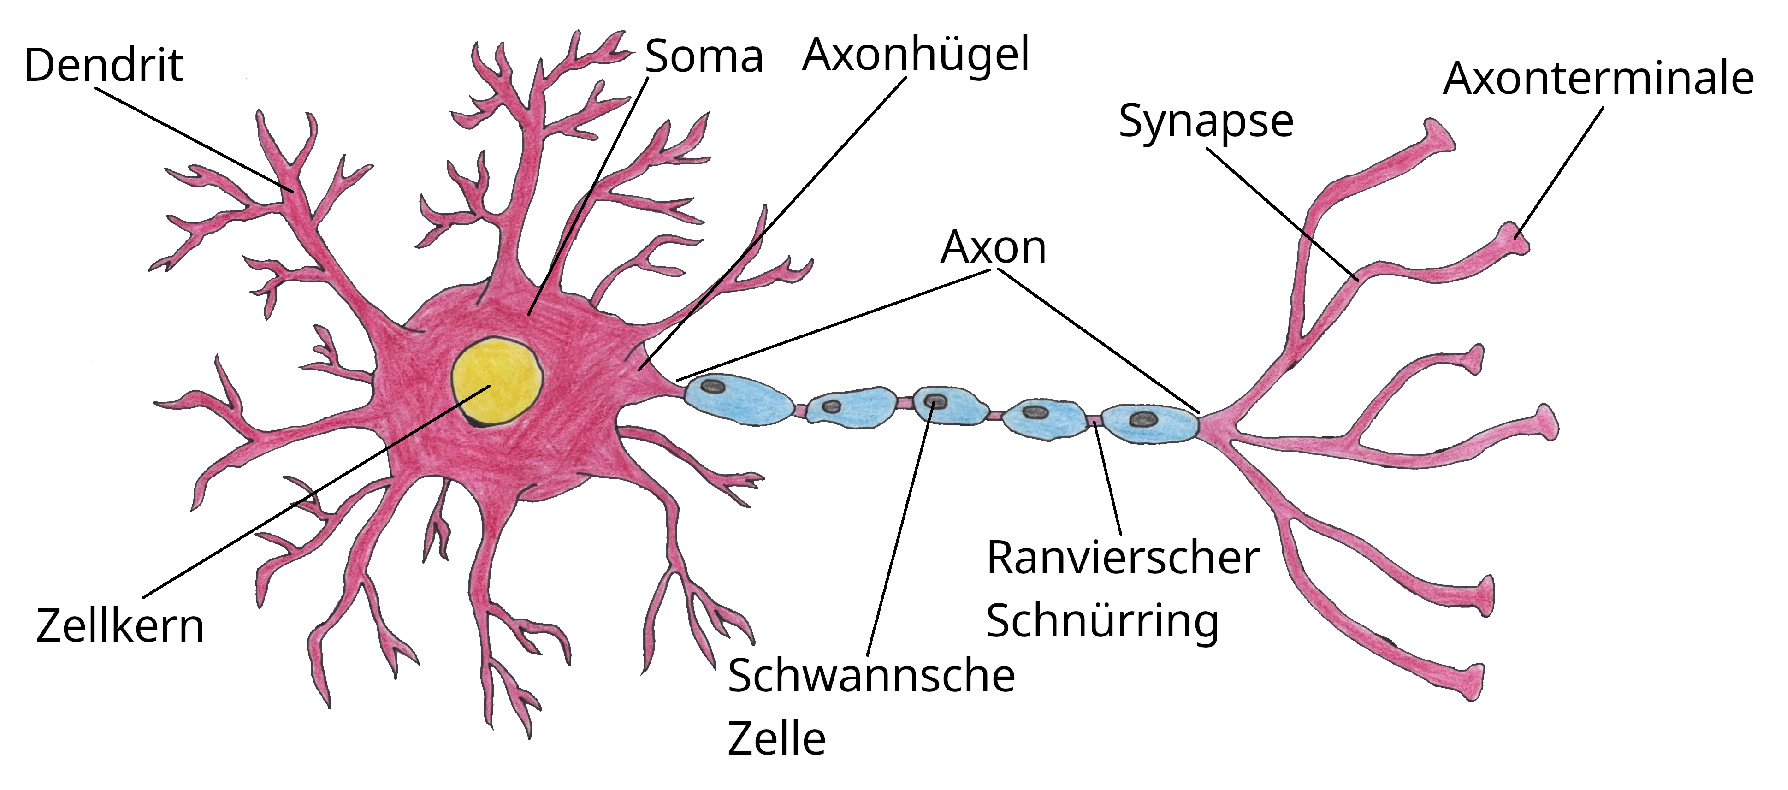
\includegraphics[width=0.8\textwidth]{content/chapter_basics/images/biological_neuron.eps}
	\centering
	\caption{Biologische Nervenzelle}
	\label{img:biological_neuron}
\end{figure}

Bei Nervenzellen werden elektrische Eingangssignale über Dendriten aufgenommen und in den Zellkern geleitet. Dort werden die eingehenden Signale zusammen geführt und es bildet sich das Aktionspotential. Übersteigt es das Schwellenpotential der Zelle, so wird das Signal über das Axon abgeleitet, die Nervenzelle \glqq \textit{feuert}\grqq.\vspace{0.2cm}

Die kleinste Einheit in künstlichen neuronalen Netzen sind die Neuronen. Sie sind den biologischen Nervenzellen nachempfunden.

\begin{figure}[!ht]
	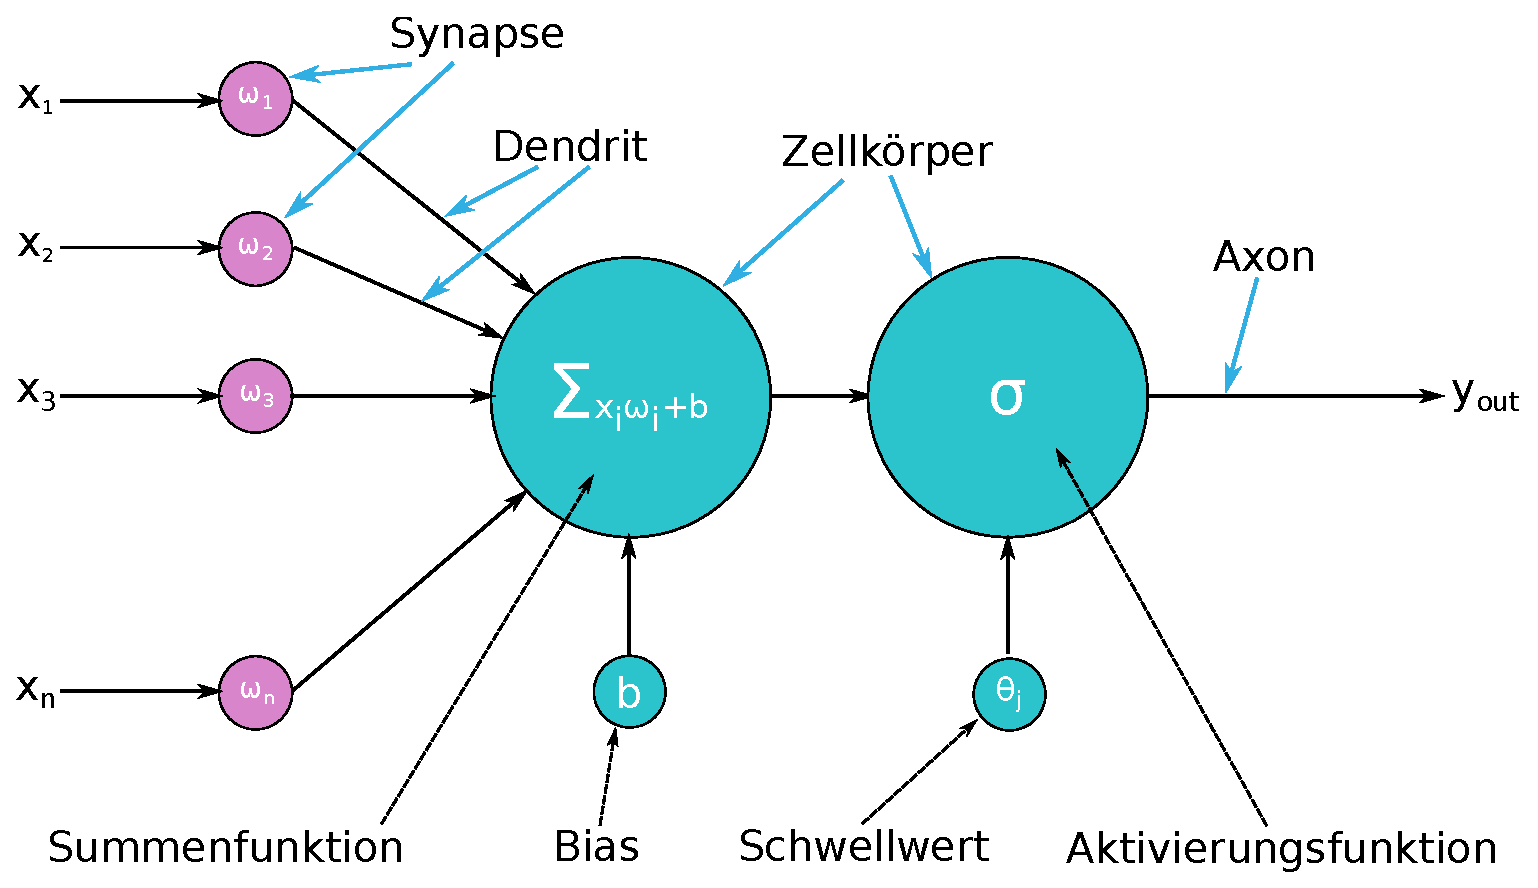
\includegraphics[width=0.8\textwidth]{content/chapter_basics/images/artificial_neuron.eps}
	\centering
	\caption{Künstliche Nervenzelle}
	\label{img:artificial_neuron}
\end{figure}

Sie haben als Eingangswert einen Vektor und als Ausgangssignal ein Skalar. Außer in der Eingabe Schicht ist jedes Eingangssignal $x_n$ ein Ausgangssignal $y_{out}$ eines anderen Neuron. Die Wichtungen der Eingangssignale modellieren den synaptischen Spalt zwischen zwei biologischen Nervenzellen. Dieser kann ebenfalls verstärkten oder hemmend wirken. Alle Eingangssignale zusammen mit den Wichtungen, werden durch die Summenfunktion aufaddiert. Im Anschluss wird das \gls{bias} mit eingerechnet. Die Formel \ref{eq:sum_function} zeigt die Summenfunktion für $n$ Eingangssignale mit Beachtung des Bias Wert.

\begin{equation} \label{eq:sum_function}
	y_{sum} = x_{1} + x_{2} + \dots + x_{n} + b
\end{equation}

Nach der Summenfunktion wird das Signal an die Aktivierungsfunktion übergeben. Diese Funktion leitet ein Signal erst weiter, wenn ein festgelegter Schwellwert überschritten wird. Die Analogie zur biologischen Nervenzelle ist das Aktionspotential, welches durch die Reize anderer Nervenzellen aufgebaut wird und wie beim künstlichen Neuron führt das Überschreiten eines Schwellenwertes dazu, dass das Neuron \glqq feuert\grqq. Die Formel \ref{eq:activation_function} zeigt das Verhalten einer \glqq Binary Step\grqq -Aktivierungsfunktion mit vorgegebenen Schwellenwert $S$.

\begin{equation}\label{eq:activation_function}
	\sigma (y_{sum}) = \left\{
	\begin{array}{cl}
		1: & y_{sum} > S \\
		0: & sonst \\
	\end{array}
	\right.
\end{equation}

Neben dieser einfachen Aktivierungsfunktion wie die \textit{Binary Step} gibt es viele weitere Aktivierungsfunktionen, beispielsweise die \textit{Sigmoidfunktion} oder \textit{ReLU (Rectified Linear Unit)} Funktion. Diese Aktivierungsfunktionen verwenden für die Berechnung immer das Ergebnis der Summenfunktion. Es gibt auch Aktivierungsfunktionen die alle Neuronen einer Schicht zur Berechnung verwenden. Zu diesen Funktionen zählen u.a. die Softmax- und die Maxout-Aktivierungsfunktion.\vspace{0.2cm}

Das eben beschriebene Neuronen-Modell ist ein einfaches Modell, welches oft in Netzen wie \textit{Feedforward Neural Netzwerke (FNN)}, \textit{Rekurrente neuronale Netze (RNNs)} oder \textit{Long Short-Term Memory Networks (LSTM)} Anwendung findet. Andere Neuronen-Modelle wie beispielsweise das \textit{Leaky-Integrate-And-Fire} Modell, finde seine Anwendung in gepulsten Netzwerken. Mit diesen mathematischen Modellen wird versucht das biologische Nervensystem nachzubilden, mit all seinen stärken und schwächen. Die Forschung hat in den letzten Jahren große Fortschritte gemacht, mit immer besser werdender Technik und Verständnis der biologischen ist das Potenzial der neuronalen Netze noch nicht erschöpft.


\subsection{Deep Learning}
Das Teilgebiet \textit{Deep Learning} versucht möglichst präzise Vorhersagen und Entscheidungen aus komplexen Daten zutreffen. Hierfür werden tiefe neuronale Netze verwendet. Das sind Netze mit vielen Hidden Layern zwischen der Ein- und Ausgabeschicht. Diese Strukturen erlauben die Verarbeitung und Analyse komplexer Datenmuster.


\section{Natural Language Processing}
Natural Language Processing ist ein Teilgebiet der Informatik und nutzt Deep Learning. NLP soll es digitalen Systemen in die Lage versetzen Texte und Sprachen zu erkennen, um diese zu verstehen und verarbeiten zu können. Dabei muss NLP die Bedeutung (Semantik) der Texte erkennen, die Grammatik und Beziehungen zwischen den Teilen der Sprache herstellen, Wortarten wie Verben, Adjektive und Nomen spezifizieren, sowie verschiedene Formen der Sprache beherrschen wie beispielsweise Prosa oder wissenschaftliches Schreiben.\vspace{0.2cm}

NLP wird aber auch in anderen Bereichen eingesetzt. Mithilfe von NLP können Bilder generiert, Suchmaschinen abgefragt, Chatbots für den Kundenservice betrieben werden und Sprachassistenten wie Amazon Alexa, MS Cortana und Apple Siri nutzen ebenfalls die NLP Techniken.\vspace{0.2cm}

Zunehmend findet NLP Einsatz im unternehmerischen Bereich. Hier werden vor allem Prozesse automatisiert um die Produktivität der Mitarbeiter zu steigern. Neben Aufgaben wie Kundensupport, Datenanalyse oder Dokumentenverwaltung kommt NLP auch in der Entwicklung von Software zum Einsatz. Hierbei werden fast alle Segmente der Entwicklung abgedeckt, von der Codegenerierung über Test und Qualitätsmanagement bis hin zur Bereitstellung.\vspace{0.2cm}

Die ersten große Erfolge hatte NLP mit neuronalen Netzen wie \textit{Feedforward Neural Networks} und \textit{Convolutional Neural Networks}, wie \cite{goldberg-2016} zeigt. Mit der Einführung von ChatGPT und BERT, wurde auch hier die neuen Transformer Modellen eingesetzt. Die Forschungen im Bereich NLP haben die großen Sprachmodelle erst ermöglicht.


\section{Large Language Model}
Die Teilgebiete Deep Learning und Natural Language Processing haben es den großen Sprachmodellen \acrshort{LLM} ermöglicht kommunikationsfähig zu werden. Sie verstehen Anfragen und können Antworten generieren. Die LLMs sind in der Lage Bilder und andere Medien wie Video oder Audio zu generieren.\vspace{0.2cm}

Die heutigen 

Diese Modelle wurden mit sehr großen Datenmengen trainiert und sind daher in der Lage natürliche Sprache zu verstehen.

\subsection{Grundlagen}
%Die großen Sprachmodelle oder Large Language Models sind darauf ausgelegt menschliche Sprache zu verstehen. Durch Textanalyse und Verarbeitung der Textbausteine durch \textit{Tokenisierung} und Vorhersage kommender Textbausteine.\vspace{0.2cm}

Die großen Sprachmodelle können menschliche Sprache arbeiten. Sie sind speziell für die Lösung  sprachbezogene Probleme geeignet, wie Textgenerierung, Klassifizierung und Übersetzung. Sie nehmen Anfragen sog. \textit{Prompts} entgegen und errechnen daraus die wahrscheinlichste Antwort. Des Weiteren können Prompts als Anweisung (instruction-tuning) oder in Dialogform (chat fine-tuning) gestellt werden. Die heutigen Sprachmodelle sind Modelle, welche die Transformer Technik verwenden.

Die grundlegende Funktionsweise der Large Language Models kann in vier Hauptkomponenten unterteilt werden,

\begin{enumerate}
	\item Tokenisierung: zerlegen der Texte in einzelne Token
	\item Embedding: Vergleiche mit anderen Vektoren und Einordnung in einer Gesamtstruktur
	\item Vorhersage: Wahrscheinlichkeit des nächsten Tokens berechnen
	\item Dekodierung: Auswahl der Ausgabestrategie
\end{enumerate}


\subsection{Grenzen und Probleme bei LLMs}
Auch wenn Künstliche Intelligenz mit ihren großen Sprachmodellen in vielen Bereichen der privaten Nutzer und in den Prozessen von Unternehmen immer präsenter wird, haben die diese auch Grenzen. Im folgen werden kurz die wichtigsten Grenzen und Probleme erläutert.

% https://www.unite.ai/de/Die-Bek%C3%A4mpfung-von-Halluzinationen-in-gro%C3%9Fen-Sprachmodellen-ist-ein-%C3%9Cberblick-%C3%BCber-modernste-Techniken/


\subsubsection{Ressourcenverbrauch}
Mit  dem Aufkommen der großen Sprachmodelle ist auch der Verbrauch an Ressourcen enorm angestiegen. Dabei stehen diese nur in einem begrenzten Maß zur Verfügung. Kleine und mittlere Unternehmen kommen hier schnell an ihre Grenzen und nutzen daher die Modelle der Anbieter wie OpenAI, Google oder Microsoft. Auch hier gilt Ressourcenbegrenzung, sodass die Modelle nicht unendlich groß werden können. Die folgenden Ressourcen, die hier genannt werden, haben direkten Einfluss auf die Modelle und deren Betrieb,

\begin{myitemize}
	\item Speicher
	\item Rechenleistung
	\item Netzwerk
	\item Energie
	\item Finanzen
\end{myitemize}

Im Lebenszyklus der großen Sprachmodelle werden Ressourcen in unterschiedlichen Mengen benötigen.\vspace{0.2cm}


\subsection{Verständnis für die LLMs}
Viele Nutzer (Privatnutzer aber auch Firmen) wissen nicht, was hinter den großen Sprachmodellen steckt oder wie diese funktionieren. Diese Unwissenheit birgt die Gefahr, dass Nutzer nicht korrekte Eingabe in die LLMs übergibt und dann die Ergebnisse der LLMs falsch interpretieren oder die LLMs nicht korrekte Aussagen trifft. Werden aufgrund dieser falschen Ergebnisse Entscheidungen getroffen, können diese enorme finanzielle und personelle Einbußen nach sich ziehen. Zudem kann es weiterhin zu Desinformation, Diskriminierung, juristische Probleme und zum Vertrauensverlust in die Technologie führen.\vspace{0.2cm}

Um diesen Problemen bei Entwicklern entgegenzuwirken, sind vor, während und nach der Einführung einer LLM zur Codeentwicklung, die Nutzer aufzuklären. Sie müssen sich im klaren sein, dass LLMs Fehler produzieren und es erforderlich ist, die Ergebnisse zu validieren. Nur so kann die ein Vertrauensverlust und eine stetige Weiterentwicklung der Modelle erfolgen.


\section{Koordinationsstrategien für LLMs}
Die Large Languarge Models haben große Leistungen auf dem Gebiet der Verarbeitung natürlicher Sprache gezeigt. Zunehmend arbeiten mehrere LLMs für diese Aufgaben zusammen. In diesem Fall spricht man von Agenten, die jeweils eine LLM darstellen können.\vspace{0.2cm}

Werden für unterschiedliche Aufgaben verschiedene Modelle verwendet, spricht man von Agenten. Ein Agent ist eine autonome Einheit. Sie ist in der Lage ihre Umwelt wahr zunehmen, Entscheidungen zu treffen und führt ihre Handlungen aus, um ein definiertes Ziel zu erreichen. Dies kann beispielsweise durch die \gls{bdi_architectur} umgesetzt werden. Jeder Agent ist auf unterschiedliche Aufgaben spezialisiert. In \cite{du-2024} werden Multi-Agenten-System mit Team aus der Softwareentwicklung verglichen und gleich gesetzt.\vspace{0.2cm}

Es gibt einige Methoden Large Language Model miteinander zu kombinieren, beispielsweise \glqq Pipeline-Architektur\grqq \ und \glqq Modular Approaches\grqq . Im Folgen Kapiteln werden die zwei Ansätze für die Zusammenarbeit von mehreren LLMs, \textit{Orchestrierung} und \textit{Multi-Agenten-System (MAS)} kurz erläutert.

\subsection{Orchestrierung von LLMs}
Bei der Orchestrierung von LLMs wird die Steuerung, der Agenten mittels eines zentralisierten Systems umgesetzt, es erfolgt eine koordinierte Nutzung. Meist wird ein Problem in Teilprobleme zerlegt und die Agenten bearbeiten Teilprobleme meist parallel. Die zentrale Steuerung entscheidet welche Teilaufgabe, welcher Agent am besten geeignet ist für die Lösung der Teilaufgabe.\vspace{0.2cm}

Die zentrale Rolle in der Orchestrierung von LLMs übernimmt dabei der Orchestrator. Dieser steuert die Aufgabenverteilung, koordiniert und kombiniert die Ergebnisse und leitet sie in die entsprechenden Agenten oder erstellt daraus die Antwort, außerdem kann er zusätzliche Aufgaben wie Fehlerbehandlung, Skalierung, Datenschutz und Sicherheit ausführen.\vspace{0.2cm}

Im Bereich der Softwareentwicklung mit Spezialisierung auf internetbasierte Anwendungen, bei der bestimmte Standards erwartet, spezielle Frameworks und Bibliotheken eingesetzt werden, könnte eine Orchestrierung bei der Umsetzung der Programmcodeerstellung wie folgt beschrieben, helfen. Bei der Lösung von Anforderungen sind nicht immer alle Agent beteiligt, vielmehr sucht der Orchestrator die jeweiligen optimalen Agenten aus.\vspace{0.2cm}

Der Orchestrator übernimmt auch hier die oben beschriebenen Aufgaben. Ein Frontend-Agent nutzt eines der großen Sprachmodelle, um Nutzeranforderungen in die Benutzeroberflächen der Anwendungen zu implementieren und könnte das Design verwalten. Gleichzeit wäre es möglich, dass dieser Agent Tools wie React.js oder Vue.js unterstützen. Für die serverseitigen Anwendungen ist der \textit{Backend-Agent} verantwortlich und verwaltet die Logik der Anwendung. Er könnte mit Frameworks wie Node.js, Express und Django umgehen. Um die Anwendung mit einer Datenbank auszustatten, kann ein \textit{Datenbank-Agent} eingesetzt werden. Er kennt verschiedenen Datenbanken wie MySQL oder PostgreSQL. Dieser verwaltet die Datenbank und deren Abfragen. Der \textit{Test-Agent} testet die Anforderung die von durch den Frontend-, Backenend- oder Datenbank-Agent umsetzt wurden.\vspace{0.2cm}

Ein letzter wichtiger Agent könnte noch der NLP-Agent sein. Dieser Agent nimmt natürliche Sprachanweisungen und Anforderungen entgegen, übersetzt diese in technische Anforderungen als Prompt für die Sprachmodelle. Die Ergebnisse der Bearbeitung werden zum Schluss von dem Agenten in eine vom Menschlichen verständliche Sprache überführt und zurückgegeben.

\subsection{Multi-Agenten-Systeme}
Multi-Agenten-Systeme (\acrshort{MAS}) bestehen ebenfalls aus mehreren Agenten. Im Gegensatz zur Orchestrierung sind Multi-Agenten-Systeme in ihrer Steuerung dezentralisiert. Alle Agenten haben unterschiedliche Lösungsansätze für ein Problem. Je nach deren Fähigkeit hat dieser auch seine ganz eigenen Ziele, welche zu den anderen Agenten entweder als \gls{collaborative} oder als \gls{competitive} ausgerichtet sind. Die Hauptarbeit zur Lösungsfindung eines Problems übernimmt der Agent, mit dem besten Lösungsansatz für das Problem. Die anderen Agenten können den ausführenden Agenten unterstützen. Um die beste Lösung zu finden, müssen die Agenten untereinander kommunizieren.  Teil der Kommunikation kann es sein, einfache Informationen austauschen, um eine gemeinsame Strategie fest zulegen oder um zu Verhandeln, welcher Agent die Lösung eines Problems übernimmt.\vspace{0.2cm}

Im Bereich der Webentwicklung mit MAS, könnte ein derartiges System wie folgt aussehen. Ein \textit{Frontend-Agent} ist für das Design und die Benutzeroberfläche verantwortlich. Hierbei erzeugt dieser Agent Ausgaben in HTML, JavaScript und CSS um die Oberflächen zu erstellen. Dazu kann er Frameworks, wie React verwenden und auf externe Designer Tool zugreifen. Ein weiterer Agent ist der \textit{Backend-Agent}, der für die serverseitige Anwendung zuständig ist. Er erstellt seine Funktionen in PHP, Python oder NodeJS. Der Backend-Agent hat Zugriff auf Frameworks und externe Bibliotheken. Der erstellt und verwaltet zudem die Datenbankoperationen (CRUD-Operations). Hinzu kommt noch ein \textit{Test-Agent}, welcher automatisierte Tests durchführt. Um die Funktionalität der Anwendung zu gewährleisten, arbeitet der Test-Agent mit dem Frontend- und Backend-Agent eng zusammen. Der Test-Agent stellt sicher, dass jegliche Codeänderung getestet wird und führt Unit-, Inetragtions- und End-to-End-Tests durch. Wird ein Fehler festgestellt, kann der Test-Agent ein Ticket erstellen oder direkt mit dem Frontend- oder Backend-Agenten kommunizieren.\vspace{0.2cm}

Ein weiterer Agent könnte ein \textit{Deploment-Agent} sein. Dieser führt automatische Depolyments in verschiedene Umgebungen (QA, Test oder Produktion) durch. Er ist in den Continuous Integration (CI) und Continuous Deployment (CD) Workflow integriert, welche die Bereitstellung auf verschiedenen Servern (VMware, Bare-Metal) und Cloud-Umgebungen (AWS, Azure, Google) bewerkstelligt. Des weitere könnten beispielsweise Security-Agent, Monitoring-Agent und Optimierungs-Agent Einsatz finden.\vspace{0.2cm}

Auch hier kann ein NLP-Agent zum Einsatz kommen und die Kommunikation zwischen Mensch und System managen.

% https://medium.com/scisharp/understand-the-llm-agent-orchestration-043ebfaead1f

%----------------------------------------------------------------

\section{Prompt Engineering}
Prompt Engineering optimiert die Antworten große Sprachmodelle, ohne Parameter, wie Bias und Gewichte des Models ändern zu müssen. Dieser Bereich hat in den letzten Jahren enorm an Bedeutung gewonnen und sich zu einer eigenen Disziplin im Bereich der Künstlichen Intelligenz entwickelt.\vspace{0.2cm}

Ein Prompt oder Anweisung muss entweder als Anweisung oder als Frage gestellt werden. Dies kann, wie in \cite{amatriain-2024} beschrieben, in Form von einer einfachen Anweisung bis hin zu detaillierten Beschreibungen oder spezifischen Aufgaben erfolgen.\vspace{0.2cm}

[Hier Beispiel von ChatGPT oder Gemini einfügen, kann als Bild]


\subsection{Prompt-Techniken}\label{subsec:prompt_technics}
Siehe Prompting Techniques Hinweise für die Optimierung von Prompts.
Die folgenden Techniken dienen dazu die Abfragen zu optimieren und somit eine bessere Antwort von den Sprachmodellen zu erhalten.


\subsection{Grenzen beim Prompt-Engineering für LLMs}
Trotz der bemerkenswerten linguistischen Leistung, stoßen große Sprachmodelle an ihre Grenzen, unter anderem wie in \cite{amatriain-2024} beschrieben,

%\section{Relevante Arbeiten}
%In \cite{zhou-2022} wird der Prompt-Optimierungsprozess als Black-Box interpretiert. Der mit minimalen Eingaben ein menschenähnliches Niveau erreichen soll.

%-------------------------------------------------------------------------------------------------------------------------------------------


%\section{Grundlagen bei der Entwicklung von Webanwendungen}
%Webanwendung

\section{Grundlagen der Webentwicklung}
In diesem Unterkapitel soll kurz auf Anforderungen der Webentwicklung eingegangen werden.


\subsection{Programmiersprachen}
Grundsätzlich kann jede Programmiersprache verwendet werden. Es gibt jedoch Programmiersprachen, die explizit für Webanwendungen entwickelt wurden und einige Funktionen mitbringen, welche die Entwicklung vereinfachen. Die meisten visuellen Anwendungen erstellen HTML (\textbf{H}yper\textbf{T}ext \textbf{M}arkup \textbf{L}anguage) Code als Grundgerüst und generieren CSS (\textbf{C}ascading \textbf{S}tyle \textbf{S}heets) Dateien für das Layout, die als Standardformatierungssprache gilt. Anwendungen die als RestAPI (\textbf{A}pplication \textbf{P}rogramming \textbf{I}nterface) fungieren liefern meist Ausgaben in Form von JSON (\textbf{J}ava\textbf{S}cript \textbf{O}bject \textbf{N}otation) aus. Neben JSON Format gibt es weitere beispielsweise XML () oder YAML (\textbf{Y}AML \textbf{A}in’t \textbf{M}arkup \textbf{L}anguage).\vspace{0.2cm}


\subsection{Entwicklung}
Bei der Entwicklung von Webseiten werden längst schon die selben Prozesse und Tools verwendet wie bei anderen Softwareprojekten. Auch hier finden Tolls wie GitLab\footnote{\href{https://about.gitlab.com/}{Gitlab} ist eine webbasierte Anwendung die Issue-Traking, CI/CD Pipelines, Dokumentation und mehr für Entwickler anbietet.} und Jenkins\footnote{\href{https://www.jenkins.io/}{Jenkins} ist ein webbasiertes Tool für die kontinuierliche Integration welches viele Build-Tools, wie Ant und Maven integriert, Testtols wie JUnit und Emma bietet, sowie Verwaltungssystem wie CVS, Subversion und Git unterstützt. Jenkins kann durch viele Plugins erweitert werden.} Anwendung. Gerade in der Entwicklung von cloudbasierten Anwendungen kommen Containertools wie Docker\footnote{Durch die Containerisierung mit \href{https://www.docker.com/}{Docker} können Anwendungen und deren Umgebungen einfach bereitgestellt und bei bedarf skaliert werden. Docker bietet eine Vielzahl von einsatzbereiten Container an, die einzeln oder in Clustern laufen können.} in Verbindung mit Kubernetes\footnote{\href{https://kubernetes.io/}{Kubernetes} ist  Orchestrierungstool für Dockercontainer das von Google entwickelt wurde. Neben den Container-Anwendungen verwaltet Kubernetes auch die Umgebung für Container, wie beispielsweise Netzwerke.} zum Einsatz. Diese Tools lassen sich hervorragend in CI/CD Pipelines integrieren. An deren Anfang steht auch hier der Entwickler, welcher durch KI Unterstützung erhalten kann.


\subsubsection{Einsatz von KI}
Der Einsatz von Künstlicher Intelligenz kann in allen Entwicklungsphasen eingesetzt werden, angefangen von der Codegenerierung über die Bereitstellung mittels Pipeline bis zur Inhaltserstellung.\vspace{0.2cm}

Der Einsatz von NL2Code steck hier noch in den Anfängen, bietet aber sehr gute Ansätze viele Aufgaben zu automatisieren oder als Werkzeug um die Entwicklung effizienter zu gestalten.\vspace{0.2cm}

Die Codegenerierung für Designelemente kann ebenso mittels NL2Code erfolgen wie komplexe Backendfunktionalitäten. Ebenso kann die vorherige Konzeption durch eine LLM erfolgen.

\section{Codeprüfungen}
Es gibt mehrere Frameworks zur Prüfung der Codequalität unter PHP. Zwei Frameworks die auch in dieser Arbeit Anwendung finden, sind die Frameworks \texttt{phpunit} und \texttt{phpmetrics}. Mit ihnen werden die, durch die LLM's generierten Codes geprüft.

\subsection{PHPUnit}
Eines der bekanntesten spezielles Framework für Unit-Tests in PHP, was als Industriestandard gilt.

\subsection{PHPMetrics}
Ein PHP Framework für die Codeanalyse, welches detaillierte Berichte über die Codequalität, Komplexität des Codes und über dessen Wartbarkeit erzeugt.

\subsection{SonarQube}
Dieses Tool zur statischen Codeanalyse und Codeprüfung. Es werden verschiedene Programmiersprachen unterstützt, darunter auch PHP.

\subsection{ESLint}
JavaScript Tool zur Syntaxfehler-Erkennung, Stil- und Codequalitätsprüfung. Mit diesem Tool kann reines JavaScript als auch Node.js überprüfen.


%\chapter{Stand der Forschung}\label{chap:state_of_research}
%%\section{Large Language Models}

\section{Methoden und Ansätze}


\section{Forschungslücken und zukünftige Forschung}


\subsection{Identifikation von Forschungslücken}


\subsection{Zukünftige Forschungsrichtungen}



\chapter{Konzeption / Design}
%Da es in deiner Arbeit primär um die *Evaluation* und *Optimierung* von LLMs für die Codegenerierung und *nicht* um die Entwicklung einer kompletten Webanwendung geht, muss das Kapitel "Konzeption / Design" diesen Fokus widerspiegeln. Es geht weniger um die Architektur einer Webanwendung als vielmehr um das Design der *Experimente* und der *Prompt-Engineering-Strategien*.

Hier ist ein Vorschlag für die Struktur des Kapitels "Konzeption / Design", der auf diesen Schwerpunkt zugeschnitten ist:

\subsubsection{Kapitel: Konzeption / Design}

Dieses Kapitel beschreibt, *wie* die im Grundlagenkapitel evaluierten LLMs für die Codegenerierung von Webanwendungen untersucht und optimiert werden. Es legt den methodischen Rahmen für die nachfolgende Implementierung (der Experimente) fest.

%**Mögliche Unterpunkte:**

%1.  **Definition der Evaluierungsziele:**
%*   Welche Aspekte der Codegenerierung sollen evaluiert werden? (z.B. Korrektheit des generierten Codes, Performance (Ausführungsgeschwindigkeit), Codequalität (Lesbarkeit, Wartbarkeit), Einhaltung von Coding Standards, Sicherheit, etc.)
%*   Welche konkreten Metriken werden zur Messung dieser Aspekte verwendet? (z.B. Anzahl der Fehler im generierten Code, Ausführungszeit in Millisekunden, statische Codeanalyse-Metriken, etc.)
%*   Dieser Abschnitt stellt sicher, dass die Evaluation messbar und reproduzierbar ist.

%2.  **Auswahl der LLMs und deren Konfiguration:**
%*   Welche LLMs werden konkret in den Experimenten verwendet? (Begründung basierend auf den Ergebnissen des Grundlagenkapitels)
%*   Welche spezifischen Parameter und Einstellungen der LLMs werden verwendet? (z.B. Temperatur, maximale Tokenanzahl, Top-p Sampling, etc.)
%*   Werden die LLMs direkt über ihre APIs angesprochen oder werden Frameworks/Bibliotheken verwendet?
%*   Dieser Abschnitt legt die experimentelle Basis fest.

%3.  **Design der Experimente:**
%*   Welche Arten von Code sollen generiert werden? (z.B. einfache HTML-Formulare, komplexe JavaScript-Funktionen, serverseitiger Code in Python/Node.js, etc.)
%*   Wie werden die Testfälle für die Evaluation generiert? (z.B. manuelle Erstellung, automatische Generierung, Verwendung von bestehenden Code-Snippets, etc.)
%*   Wie groß ist der Umfang der Testfälle? (Anzahl der zu generierenden Code-Snippets)
%*   Wie werden die Ergebnisse der LLMs verglichen? (z.B. Vergleich mit Referenzcode, manuelle Überprüfung, automatische Tests, etc.)
%*   Dieser Abschnitt ist zentral für die Arbeit, da er die methodische Vorgehensweise der Evaluation beschreibt.

%4.  **Konzeption des Prompt-Engineerings:**
%*   Welche Strategien für das Prompt-Engineering werden untersucht? (z.B. Few-Shot-Prompting, Chain-of-Thought-Prompting, Verwendung von Code-Kommentaren als Prompts, etc.)
%*   Wie werden die Prompts aufgebaut sein? (z.B. klare Anweisungen, Beispiele, Kontextinformationen, etc.)
%*   Werden verschiedene Prompt-Varianten für die gleichen Code-Generierungsaufgaben verwendet, um deren Einfluss auf die Ergebnisse zu untersuchen?
%*   Dieser Abschnitt ist besonders wichtig, da er sich mit der Optimierung der LLMs durch Prompt-Engineering beschäftigt.

%5.  **Evaluationsumgebung:**
%*   Welche Hardware und Software werden für die Experimente verwendet? (z.B. CPU, GPU, Betriebssystem, Programmiersprachen, Bibliotheken, etc.)
%*   Wie wird die Reproduzierbarkeit der Experimente sichergestellt? (z.B. Verwendung von Versionskontrolle, Dokumentation der Umgebung, etc.)

\subsubsection{Beispiel}

Im Grundlagenkapitel wurden verschiedene LLMs hinsichtlich ihrer Fähigkeit zur Generierung von JavaScript-Code evaluiert. Im Konzeptionskapitel könnte nun festgelegt werden, dass drei dieser LLMs (z.B. Codex, GPT-3.5-turbo, Gemini) anhand von 50 verschiedenen JavaScript-Funktionen evaluiert werden. Die Funktionen sollen unterschiedliche Komplexitätsgrade aufweisen (einfache Funktionen, Funktionen mit Schleifen und Bedingungen, Funktionen mit DOM-Manipulation). Für jede Funktion werden drei verschiedene Prompt-Varianten erstellt: ein einfacher Prompt, ein Prompt mit Code-Kommentaren als Kontext und ein Prompt mit zwei Beispiel-Funktionen (Few-Shot-Prompting). Die Korrektheit des generierten Codes wird durch automatische Unit-Tests überprüft.

\subsubsection{Abgrenzung zur Implementierung}

Die Implementierung setzt die im Konzeptionskapitel definierten Experimente und Prompt-Engineering-Strategien konkret um. Hier wird der Code geschrieben, die Experimente durchgeführt und die Ergebnisse gesammelt. Das Konzeptionskapitel dient als detaillierte "Blaupause" für die Implementierung.

Durch diese Struktur wird deutlich, dass es in deiner Arbeit um die systematische *Untersuchung* und *Verbesserung* der LLM-basierten Codegenerierung geht und nicht um die Entwicklung einer konkreten Webanwendung. Das Kapitel "Konzeption / Design" legt den methodischen Grundstein für diese Untersuchung.

In diesem Kapitel werden die Rahmen- und Randbedienungen für das methodische Vorgehen der Evaluation großer Sprachmodelle für die Codegenerierung von webbasiertem Code festgehalten. Dies umfasst die Festlegung der verwendeten LLMs, die geprüfte Programmiersprachen, Framework zur Erstellung und Auswertung der Tests und Systeme für die Bereitstellung und Verarbeitung der Ergebnisse. Die Evaluierung der Modelle erfolgt in deutscher Sprache, was die Prompts und die Tests betrifft. Allein die Methodenbezeichnung ist in englischer Sprache.

\section{Definition der Evaluierungsziele}
%*   Dieser Abschnitt stellt sicher, dass die Evaluation messbar und reproduzierbar ist.

%*   Welche Aspekte der Codegenerierung sollen evaluiert werden? (z.B. Korrektheit des generierten Codes, Performance (Ausführungsgeschwindigkeit), Codequalität (Lesbarkeit, Wartbarkeit), Einhaltung von Coding Standards, Sicherheit, etc.)
Ausgehend von den in Kapitel \ref{sec:goals_of_the_work} gestellten Ziele dieser Arbeit, werden hier das Konzept und das Design für die Evaluation beschrieben. Wie werden die Ziele erreicht und welche Komponenten sind dazu erforderlich, um die Daten zu erheben und auszuwerten.\vspace{0.2cm}

Die Evaluation soll zeigen, ob die generierten Codes korrekt funktioniert und es nicht zu Laufzeitfehlern oder Deadlocks kommt. Des Weiteren wird evaluiert, ob der Code den gängigen Programmierstil entsprechen und welche Qualität der generierte Code ausweist. Hier liegt vor allen der Fokus auf Lesbarkeit und Einhaltung von Codingstandards. Als letzter Punkt soll die Dokumentation innerhalb des Codes geprüft werden. Je besser diese Ausfällt je leichter sind spätere Refactorings möglich.\vspace{0.2cm}

Was nicht im Fokus liegt und in den Test vernachlässigt wird, sind die Performance der Modelle und die Architekturen der Systeme auf denen die Modelle laufen. Es geht in erster Linie um den generierten Code und dessen Brauchbarkeit für die reelle Verwendung in der Praxis.\vspace{0.2cm}

%*   Welche konkreten Metriken werden zur Messung dieser Aspekte verwendet? (z.B. Anzahl der Fehler im generierten Code, Ausführungszeit in Millisekunden, statische Codeanalyse-Metriken, etc.)
Für die Messung der Fehler wird die \texttt{pass@k} Metrik angewandt. Diese Metrik baut auf einen mitgelieferten Test für jedes Problem auf. Der Test zusammen mit dem generierten Code ergeben einen ausführbaren Code. Jeder Test wird in einer Liste notiert und dazu das Ergebnis ob positiv oder negativ. Daraus kann dann mit der \texttt{pass@k} Metrik die repräsentative Zuverlässigkeit des Modells für jedes Problem und für das Modell errechnet werden.\vspace{0.2cm}

Für die erweiterte Messung des PHP Codes kommt das Tool \texttt{phpmetrics} zum Einsatz. \texttt{phpmetrics} liefert eine Vielzahl an Metriken,mit der der Code analysiert werden kann. Bei diesem Tool liegt der Fokus auf die Ergebnisse von \texttt{Cyclomatic Complexity}, mit der die Komplexität des Codes gemessen wird. Auf den \texttt{Maintainability Index} zur Auswertung der Wartbarkeit. Diese ermittelt wie aufwändig es zukünftig ist den Code zu erweitern und bewertet die Lesbarkeit. Ein weiterer Parameter welcher hilft die Komplexität zu bewerten, ist der \texttt{Logical Lines of Code} Parameter. Ein weiteres Indiz zur Wartbar- und Lesbarkeit ist der \texttt{Method Length} Parameter. Ein weiterer Parameter zur Bewertung der Lesbarkeit ist der Parameter \texttt{Numbers of Parmeters}. Diese gibt die Anzahl der Parameter welche in die Methode übergeben werden. Eine hohe Anzahl kann ein Indiz dafür sein, das der Code schwerer zu lesen ist. Zur Bewertung der Dokumentation wird der Parameter \texttt{Comment Density} herangezogen.
Mithilfe eines Python-Skripts wird der generierte Code mit \texttt{phpmetrics} evaluiert.\vspace{0.2cm}

(SonarQube, wenn die Zeit es noch erlaubt)

Mit dem SonarQube steht ein Auswertungstool zur Verfügung, welches neben qualitativen Codeanalyse noch eine Sicherheitsanalyse des Codes durchführt und die technischen Schulden ermittelt. Somit ist SonarQube eine Ergänzung zu \texttt{phpmetrics}. SonarQube wird eine lokale VM ausgeführt und mittels Integration werden die generierten Codes an den Server übermittelt.\vspace{0.2cm}

Beide Verfahren \texttt{phpmetrics} und \texttt{SonarQube} benötigen für die Analyse Dateien. Somit müssen die Ergebnisse erst als Datei gespeichert werden, bevor die Tools mit der Analyse beginnen.

%---------------------------------------------------------------------------------------------------


\section{Auswahl der LLMs und deren Konfiguration}
%*   Dieser Abschnitt legt die experimentelle Basis fest

%*   Welche LLMs werden konkret in den Experimenten verwendet? (Begründung basierend auf den Ergebnissen des Grundlagenkapitels)
Für die Evaluation werden experimentell einige freie und kommerzielle Modelle ausgewählt und miteinander verglichen. Hauptsächlich wurden bei den freien Modellen, jene ausgewählt welche den Fokus auf die Codegenerierung legen und mit diesem Argument beworben werden. Als Referenz sollen die kommerziellen Modelle dienen, da durch hier weite Verbreitung und breite Nutzer ihre Daten stetig erweitern und die Entwicklung vorantreiben.\vspace{0.2cm}

Im Folgenden werden die ausgewählten LLMs kurz vorgestellt und warum diese gewählt wurden. Die Reihenfolge stellt an dieser Stelle keine Wertung der LLM oder über deren generierten Inhalte dar.\vspace{0.2cm}

Das \textbf{Qwen2.5-Coder}-Modell zeichnet sich durch seine spezialisierte Architektur für die Codegenerierung aus. Trainiert, um sowohl syntaktisch korrekten als auch funktional hochwertigen Code zu produzieren, integriert es fortschrittliche Mechanismen zum Kontextverständnis und semantisch sinnvolle Ausgabe. Es findet Anwendung in verschiedenen Bereichen der Softwareentwicklung, insbesondere in der Web- und Anwendungsprogrammierung. Die Qwen2.5-Coder Modellbeschreibung ist \cite{qwen-2024} und \cite{hui-2024} entnommen und wird in den Arbeiten vertieft.\vspace{0.2cm}

\textbf{Deepseek-Coder-V2} ist die zweite Generation der Deepseek-Coder-Reihe und bietet verbesserte Fähigkeiten zur Codegenerierung und -optimierung. Das Modell nutzt fortschrittliche Suchalgorithmen, um präzisere und effizientere Codestücke zu erstellen. Es ist insbesondere für seine hohe Genauigkeit bei der Generierung komplexer Algorithmen und Datenstrukturen bekannt. Die Modellbeschreibung ist unteranderem aus \cite{deepseek-ai-2024} und \cite{cui-2024} entnommen. Des Weiteren wird in beiden Arbeiten das Modell mit verschiedenen Open-Source und Close-Source Modellen verglichen.\vspace{0.2cm} 

Die Modelle \textbf{Llama 3.1-Claude} und \textbf{Llama 3.1} gehören mit 8 Milliarden Parametern zu den kleineren Modellen von MetaAI. Beide Modelle basieren auf dem LLama3.1 Modell, das Llama3.1-Claude ist aber mit anderen Systemaufforderungen erstellt wurden. Hierfür wurden die Systemaufforderungen vom Claude Sonnet 3.5 der Firma Anthropic’s verwendet, nachzulesen unter \cite{ollama_page_llama31_claude}. Ein ähnliches Modell ist auf Hugging Face veröffentlicht \cite{huggingface_page_llama31_claude}. Eine Modelcard mit weiteren Informationen zum Modell ist unter \cite{meta-llama-no-date} zu finden.\vspace{0.2cm}

\textbf{Mistral} ist ein modernes leistungsfähiges Sprachmodell, welches nicht speziell für die Codegenerierung und -analyse entwickelt wurde. Es verwendet fortschrittliche Transformer-Architekturen und ist für eine Vielzahl von Aufgaben einsetzbar. Darunter fallen beispielsweise natürliche Sprachverarbeitung, Textzusammenfassungen, maschinelle Übersetzung und Textklassifizierung. Dieses Modell ausgewählt, um ein Modell zu evaluieren, welches nicht speziell auf Codegenerierungsaufgaben trainiert wurde. In der Arbeit \cite{eberhardinger-2024} wurde Mistral, mit verschiedenen Modelle zur Spielecodegenerierung verglichen. Während in \cite{quan-2024} eine Evaluation für natürlichsprachlicher Erklärungen, Mistral mit anderen Modellen verglichen wurde.\vspace{0.2cm}

%\textbf{ChatGPT 3.5} und das Nachfolgemodell \textbf{ChatGPT 4}, entwickelt von OpenAI, sind vielseitig einsetzbare Close-Source Modelle. Neben allgemeinen textuellen Einsatzgebieten kann es für die Codegenerierung eingesetzt werden. Seit November 2022 ist das Modell ChatGPT 3.5 für alle kostenlos nutzbar und wird von sehr vielen Nutzer eingesetzt. Mit diesen Daten werden neue Modelle, wozu auch ChaGPT 4 zählt ständig neu trainiert. Dadurch werden die Modelle immer besser. Die Fallstudie \cite{ahmed-2025} die Bewertung des Nutzens von ChatGPT 4 für die Gestaltung einer barrierefreien Webseite. Eine Übersicht über die Modelle ist unter \cite{openai_model_overview} einsehbar.\vspace{0.2cm}

Mit \textbf{Gemini 1.5} präsentiert Google ein Modell zur Verarbeitung von natürlicher Sprache und stellt es zur freien Nutzung zur Verfügung. Genau wie ChatGPT nutzt auch Google die Nutzereingaben, um neue Modelle zu trainieren, was zur Weiterentwicklung für und somit zum neuen Modell \textbf{Gemini 2}. Wie in \cite{siam-2024} beschrieben, setzen auch die Gemini Modelle die Transformer-Architektur ein, was sie dazu befähigt, komplizierte Sprachmuster zu erkennen und präzise Vorhersagen zutreffen. In \cite{siam-2024} wird Gemini 1.5 mit Aufgaben zur Codegenerierung mit ChatGPT und Copilot vergleichen. Nach \cite{elgedawy-2024} kann sich das Gemini-Ultra-Modell beim MMLU-Benchmark sogar mit menschlichen Experten messen und erschließt eine breite Palette von Anwendungsbereichen. Hier wurden die Fähigkeiten zur Codegenerierung an Sicherheitsfragen im E-Commerce Bereich getestet. Ein Überblick über die Gemini Modelle ist unter \cite{google_gemini_model_overview} zu finden.\vspace{0.2cm}

Neben den genannten Quellen sind die Herstellerseite eine gute Quelle weiterführende Informationen einzuholen.\vspace{0.2cm}

Die Tabelle \ref{tab:selected_llms} zeigt zusammenfassend die ausgewählten Modelle.\vspace{0.2cm}

\begin{table}[!ht]
	\begin{tabular}{|l|c|c|c|c|c|l|}
		\hline
		\textbf{Modell} & \textbf{Parameter} & \textbf{Größe} & \textbf{Sprache} & \textbf{offen} & \textbf{Ausführung}  & \textbf{Benchmark} \\
		\hline
%		Qwen2.5-coder     &  32b &  19 GB & German & X & lokal/HF  & HE-XL \\
		%		CodeGeeX          &  9B & German &  & & lokal & HE-XL \\
%		Deepseek-coder-V2 &  16b & 8,9 GB & German & X & lokal/Ollama  & HE-XL \\
		Llama3.1-Claude   &   8b & 4,7 GB & German & X & lokal/Ollama  & HE-XL \\
		Llama3.1          &   8b & 4,7 GB & German & X & lokal/Ollama  & HE-XL \\
		Llama3.2          &   3b & 2,0 GB & German & X & lokal/Ollama  & HE-XL \\
%		Codellama         &  13b & 7,4 GB & German & X & lokal/Ollama  & HE-XL \\
		Mistral Small     &  22b &  12 GB & German & X & lokal/Ollama & HE-XL \\
%		ChatGPT3.5-turbo  & k.A. &   k.A. & German & - & online & HE-XL \\
		ChatGPT4-turbo    & k.A. &   k.A. & German & - & online & HE-XL \\
		Gemini 1.5 Pro    & k.A. &   k.A. & German & - & online & HE-XL \\
%		Gemini 2 Pro      & k.A. &   k.A. & German & - & online & HE-XL \\
		%		Opus              & & & German &  & online & HE-XL \\
		%		Claude 3          & &  German & & & online & HE-XL \\
		\hline
		%		\multicolumn{7}{|l|}{In Planung, wenn ich es schaffe} \\
		%		\hline
		%		Llama3.3          & 70b &  43 GB & German & X & lokal  & HE-XL \\
		%		\hline
%		\multicolumn{7}{|l|}{HF: Hugging Face} \\
		\multicolumn{7}{|l|}{HE-XL: HumanEval-XL Benchmark} \\
		\hline
	\end{tabular}
	\caption{Auswahl der LLMs für die Evaluierung}
	\label{tab:selected_llms}
\end{table}

%*   Welche spezifischen Parameter und Einstellungen der LLMs werden verwendet? (z.B. Temperatur, maximale Tokenanzahl, Top-p Sampling, etc.)
Die Einstellung für die Abfragen der Probleme wurden bei allen Modellen identisch gewählt.\vspace{0.2cm}

Für die Abfragen der Testprobleme wurde eine \textit{temperature} von $0.2$ gewählt. Ein niedriger Wert veranlasst die Modelle deterministischere und standardisierte Antworten zu geben und verhindert Kreativität und Zufälligkeit. Die Generierung von Programmcode soll konsistenten und präzisen Code liefern.\vspace{0.2cm}

Ein hoher \textit{top\_p} Wert verlangt von den Modellen eine Antwort die mit hoher Wahrscheinlichkeit richtig ist. Für die Codegenerierung sollten die wahrscheinlichsten und syntaktisch korrekten Token angewandt werden. Für die Abfragen wird hier ein Wert von $0.95$ angesetzt.\vspace{0.2cm}

Die maximale Anzahl Token sollte bei der Generierung von Code zwischen 20 und 1000 Token eingestellt werden, je nach Umfang der Antworten. Da hier nicht nur die Funktionsfähigkeit geprüft wird, sondern auch Struktur und Coding-Standards wird ein hoher Wert ausgewählt, sodass beispielsweise Kommentare ebenfalls enthalten sind können. Somit wird \textit{max\_token} auf sechshundert festgelegt.\vspace{0.2cm}

In der Tabelle \ref{tab:params_for_llms} sind die Werte in übersichtlicher kurzer Form noch einmal dargestellt.

\begin{table}[!ht]
	\begin{tabular}{|l|c|c|c|}
		\hline
		\textbf{Modell} & \textbf{Temperatur} & \textbf{max. Tokenanzahl} & \textbf{Top-p Sampling} \\
		\hline
		Qwen2.5-coder     & 0.2 & 600 & 0.95 \\
		Deepseek-Coder-v2 & 0.2 & 600 & 0.95 \\
		Llama3.1-Claude   & 0.2 & 600 & 0.95 \\
		Llama3.2          & 0.2 & 600 & 0.95 \\
%		Codellama         & 0.2 & 600 & 0.95 \\
		Mistral Small     & 0.2 & 600 & 0.95 \\
%		ChatGPT3.5-turbo  & 0.2 & 600 & 0.95 \\
		ChatGPT4-turbo    & 0.2 & 600 & 0.95 \\
		Gemini 1.5 Pro    & 0.2 & 600 & 0.95 \\
%		Gemini 2 Pro      & 0.2 & 600 & 0.95 \\
		\hline
	\end{tabular}
	\centering
	\caption{Einstellungen der Modellparameter}
	\label{tab:params_for_llms}
\end{table}

Hinzu kommen weitere Parameter für die Modelle. Unter anderem wird der Parameter \textit{do\_sample} auf $False$ gesetzt, was die Modelle veranlasst den wahrscheinlichsten folgenden Token zu wählen und ein deterministisches Verhalten fördert. Ein weiterer Parameter ist \textit{return\_full\_text} der ebenfalls auf $False$ gesetzt wird. Dadurch werden nur die neu generierten Tokens zurückgegeben, was die Relevanz der Antworten fördert.\vspace{0.2cm}

%*   Werden die LLMs direkt über ihre APIs angesprochen oder werden Frameworks/Bibliotheken verwendet?
Alle Prompts welche die Probleme enthalten, werden mit Python Skripten abgefragt. Dies gilt für die offenen lokalen wie auch für die kommerziellen Modelle. Die Abfragen werden jeweils an die entsprechenden APIs abgesetzt. Als Frameworkfür die Abfragen der lokalen Modelle, kommt das Python \texttt{langchain} Framework zu Einsatz. Für die Modelle der Gemini-Reihe wird die Google eigene Bibliothek, \texttt{google.genai} verwendet. Dasselbe trifft für die Modelle von OpenAI zu. Hier kommt die Python Bibliothek \texttt{openai} zum Einsatz.

%---------------------------------------------------------------------------------------------------


\section{Design der Experimente}
%*   Dieser Abschnitt ist zentral für die Arbeit, da er die methodische Vorgehensweise der Evaluation beschreibt.
Das Experiment wird mit dem HumanEval-XL Benchmark durchgeführt. Dieser Benchmark besteht aus einer Reihe von 80 Tests in verschiedenen Programmiersprachen, die wie folgt aufgebaut sind,

\begin{myitemize}
	\item \textbf{task\_id}: Kennung der Datenprobe
	\item \textbf{prompt}: Anfrage für das Modell, Funktionsheader und Docstring
	\item \textbf{entry\_point}: Einstiegspunkt für den Test
	\item \textbf{test}: Test für die geforderte Funktion
	\item \textbf{description}: Beschreibung der Aufgabe
	\item \textbf{language}: Kennung der Programmiersprache
	\item \textbf{canonical\_solution}: Lösung für das Problem
	\item \textbf{natural\_language}: Ländersprache in der Datei
\end{myitemize}

Die Abbildung \ref{img:code_generation_humaneval} zeigt den Aufbau und damit alle wichtigen Bereiche des Benchmark-Tests.\vspace{0.2cm}

\begin{figure}[!ht]
	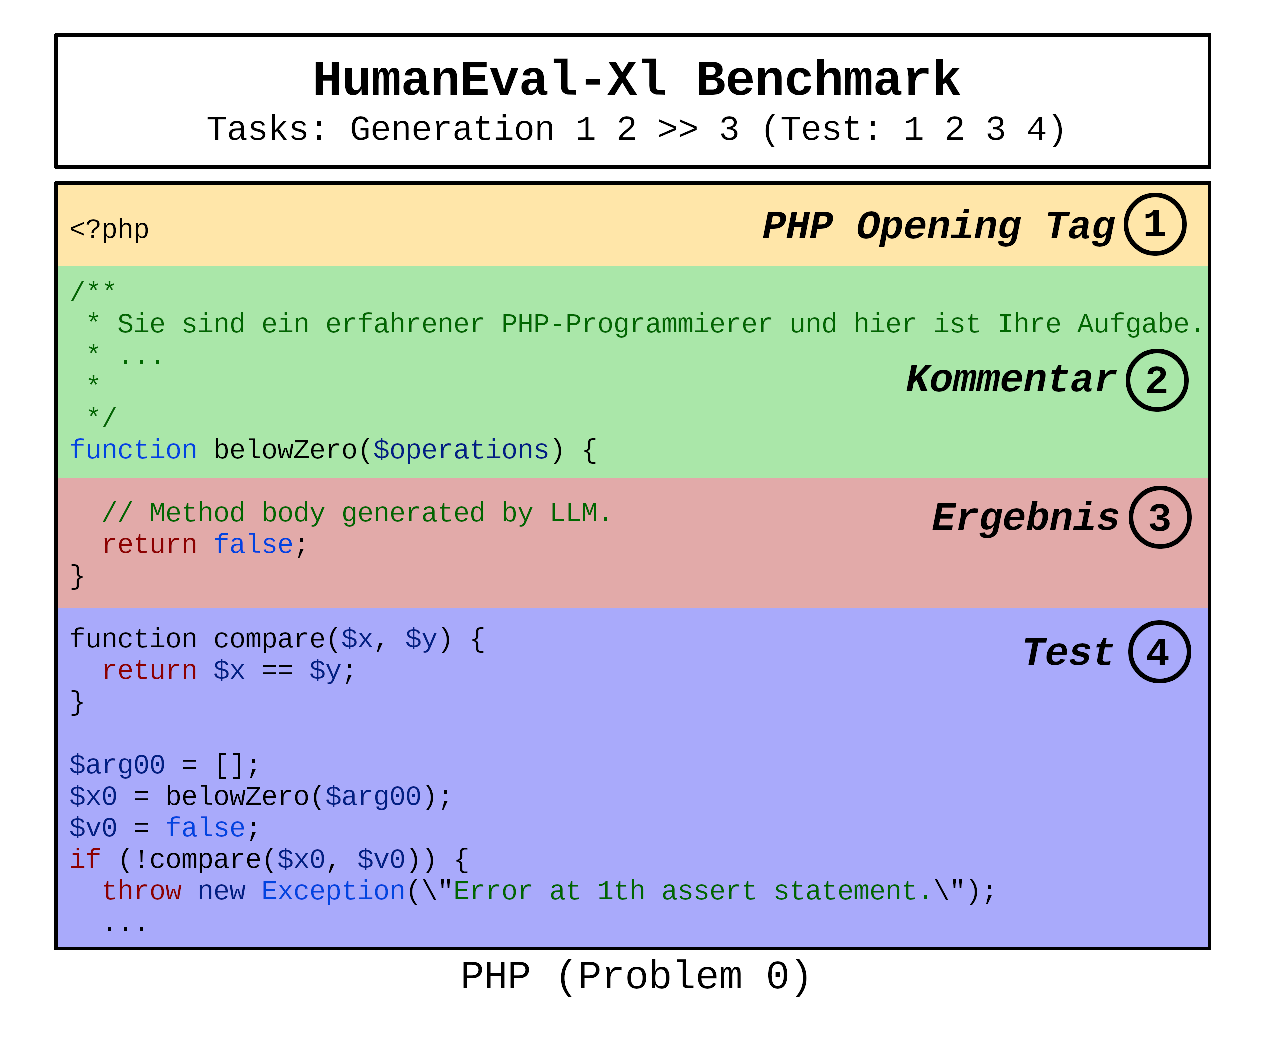
\includegraphics[width=0.8\textwidth]{content/chapter_intruduction/images/code_generation_humaneval_x.eps}
	\centering
	\caption{Codegeneration}
	\label{img:code_generation_humaneval}
\end{figure}

%*   Welche Arten von Code sollen generiert werden? (z.B. einfache HTML-Formulare, komplexe JavaScript-Funktionen, serverseitiger Code in Python/Node.js, etc.)
Um die Modelle zu evaluieren und ihre Fähigkeiten hinsichtlich der im Web vorherrschenden Programmiersprachen zu untersuchen, werden die Tests in den Programmiersprache(n) PHP (und JavaScript) vorgenommen. Dafür sollen die Modelle mehrfach einfache Funktionen generieren.\vspace{0.2cm}

%*   Wie werden die Testfälle für die Evaluation generiert? (z.B. manuelle Erstellung, automatische Generierung, Verwendung von bestehenden Code-Snippets, etc.) Wie groß ist der Umfang der Testfälle? (Anzahl der zu generierenden Code-Snippets)
Der Benchmark liefert die Tests mit. Dazu werden bereits in den Prompts die Namen der Methoden und die zu übergebenen Parameter angegeben, welche zu erstellen ist. Der jeweilige Test verwendet dann diesen Namen und übergibt die geforderten Parameter. Das Listing \ref{lst:example_prompt_test_by_humaneval_benchmark} zeigt ein Beispiel für einen mitgelieferten HumanEval-XL Test.

\begin{lstlisting}[language=php,caption={Beispiel für einen Test aus dem HumanEval-XL Benchmark},label=lst:example_prompt_test_by_humaneval_benchmark]
function compare($x, $y) {
	return $x == $y;
}
$arg00 = [3, 1, 2, 4, 5];
$x0 = median($arg00);
$v0 = 3;
if (!compare($x0, $v0)) {
	throw new Exception(\"Error at 1th assert statement.\");
}
\end{lstlisting}


%*   Wie werden die Ergebnisse der LLMs verglichen? (z.B. Vergleich mit Referenzcode, manuelle Überprüfung, automatische Tests, etc.)
Um die Modelle untereinander zu vergleichen, bekommen alle Modelle dieselben Prompts. Von jedem Prompt werden pro Modelle zehn Varianten erstellt. Die Ergebnisse werden in einer Liste chronologisch gespeichert. Diese Ergebnisse werden dann mittels der \texttt{pass@k} Metrik geprüft.

%---------------------------------------------------------------------------------------------------


\section{Konzeption des Prompt-Engineerings}
%*   Welche Strategien für das Prompt-Engineering werden untersucht? (z.B. Few-Shot-Prompting, Chain-of-Thought-Prompting, Verwendung von Code-Kommentaren als Prompts, etc.)
Die Prompts im HunamEval-XL Benchmark sind als Few-Shot-Prompts verfasst. Sie neben der eigentlichen Aufgabe sind noch Beispiel für die Eingabedaten und erwarteten Ergebnisse angegeben. Das Listing \ref{lst:example_prompt_by_humaneval_benchmark} zeigt ein Beispiel für einen Prompt.

\begin{lstlisting}[language=php,caption={Prompt Beispiel für  eine Aufgabe aus dem HumanEval-XL Benchmark},label=lst:example_prompt_by_humaneval_benchmark]
<?php

/**
* Sie sind ein erfahrener PHP-Programmierer und hier ist Ihre Aufgabe.
* Gib den Median der Elemente in der Liste l zurück.
* >>> median([3, 1, 2, 4, 5])
* 3
* >>> median([-10, 4, 6, 1000, 10, 20])
* 15.0
*
*/
function median($l){
\end{lstlisting}

%*   Wie werden die Prompts aufgebaut sein? (z.B. klare Anweisungen, Beispiele, Kontextinformationen, etc.)
Alle Prompts im Benchmark sind als Code-Kommentare aufgebaut. Als letzte Zeile ist der Methodenname angegeben. Somit soll sichergestellt werden, dass die erstellten Tests funktionieren.\vspace{0.2cm}

\begin{tcolorbox}[
	enhanced,
	colback=red!5!white,
	colframe=red!75!black!50,
	title= Mein roter Faden
	]
	Hier kommen noch Optimierungsangaben, die stehen zurzeit nicht fest.
\end{tcolorbox}

%*   Werden verschiedene Prompt-Varianten für die gleichen Code-Generierungsaufgaben verwendet, um deren Einfluss auf die Ergebnisse zu untersuchen?


%*   Dieser Abschnitt ist besonders wichtig, da er sich mit der Optimierung der LLMs durch Prompt-Engineering beschäftigt.

%---------------------------------------------------------------------------------------------------


\section{Evaluationsumgebung}
%*   Welche Hardware und Software werden für die Experimente verwendet? (z.B. CPU, GPU, Betriebssystem, Programmiersprachen, Bibliotheken, etc.)
Die freien Modelle laufen auf einem Debian 12 System, welches mit 16 CPUs und 32 GB RAM ausgestattet ist. Um zusätzlichen Speicher zu erhalten, wurde eine 100 GB Swap Partition genutzt. Für die Bereitstelle ist das freie Framework Ollama zum Einsatz gekommen.\vspace{0.2cm}

Auf die kommerziellen Modelle kann kein Einfluss auf die Systeme genommen werden.

%*   Wie wird die Reproduzierbarkeit der Experimente sichergestellt? (z.B. Verwendung von Versionskontrolle, Dokumentation der Umgebung, etc.)



\chapter{Implementierung}\label{chap:implementation}
\begin{tcolorbox}[
	enhanced,
	colback=red!5!white,
	colframe=red!75!black!50,
	title= Mein roter Faden
	]
	Wichtigsten Aspekte und Schritte der Implementierung. Aufbau und Struktur evtl. Programme, wichtige techn. Entscheidungen (Nicht den gesamten Quellcode abbilden, wenn überhaupt dann im Anhang). Einbinden, nur wenn,

	\begin{enumerate}
		\item Nur erklärungsbedürftigen Code ca. 5-20 Zeilen.
		\item Für Nachvollziehbarkeit.
		\item Kommentare für Erklärung.
		\item Keine Standards oder Bibliotheken.
		\item Komplexe Klassen/Strukturen besser beschreiben.
		\item Alternativen:
		\begin{itemize}
			\item Pseudocode.
			\item Diagramme.
			\item Erklären der Logik durch Text.
		\end{itemize}
	\end{enumerate}

	Max. 10-12\% des Kapitels, Rest in Anhang.
\end{tcolorbox}

\section{Lokale Modelle}
Um die Modelle testen zu können ist es erforderlich diese auf geeignete Hardware bereitzustellen. Die zur Verfügung stehende Hardware erlaubt die Bereitstellung von Modellen bis etwa 70b, wobei hier eine Modellquantisierung angewandt werden muss, sodass die Speichergröße etwa eine maximale Größe von 25 bis 30 Gigabyte nicht überschreitet.\vspace{0.2cm}

Ein Tool zur Verwaltung und Ausführung von LLMs ist Ollama. Ollama bieten eine Reihe von Modellen an, die den zur vor genannten Bedingungen entsprechen. Ein weiterer Vorteil für Ollama ist Unterstützung der Programmiersprache Python. Diese wird verwendet, um mit den Modellen zu interagieren und die Ergebnisse zu evaluieren.


\subsection{Bereitstellen er Modelle}
Für das Testen der lokalen Modelle wird das Ollama Framework angewandt. Dies ermöglicht eine Anbindung an einer API, welche sich beispielsweise mittels Python abfragen lässt. Auf dieser Weise lassen sich Modelle von der \href{https://ollama.com/search}{Ollama Modell} Seite testen. Dazu wird Ollama auf dem Server installiert und konfiguriert, siehe Anhang \ref{sec:install_config_ollama_local}. Nach dem Download stehen die Modelle zur Verfügung und mittels der integrierten API können Interaktionen erfolgen. Das Listing \ref{lst:python_connect_ollama} zeigt die erforderlichen und optionalen Parameter für eine einfache Interaktion mit einem Ollamaserver notwendig sind.\vspace{0.2cm}

\begin{lstlisting}[
	language=Python,
	caption={Interaktion in Python mit Ollamaserver},
	label=lst:python_connect_ollama
]
from langchain_ollama.llms import OllamaLLM

model = OllamaLLM(
    base_url="192.168.1.56:11434", # required
    model="deepseek-r1:32b", # required
    temperature=0.2, top_p=0.95, num_predict=2048, # optional
)
\end{lstlisting}

Zusätzlich bietet Ollama die Möglichkeit ein grafisches Tool zum Testen zu installieren. Mit Open WebUI wird ein Browser basierendes Toll eingesetzt, dass auf dem Ollama-Server aufgesetzt wird. Nach der Installation ist das Tool einsatzbereit und im lokalen Netzwerk, unter http://<<server-ip>>:<<webui-port>> erreichbar. Die Installation wird im Anhang \ref{sec:open_webui} beschrieben.


%\subsection{Modellbereitstellung als Datei}
%Eine zweite Methode zur Bereitstellung von Modellen die für diese Arbeit Verwendung findet, ist die direkte Nutzung als lokale Datei. Diese können dann direkt angesprochen werden, in dieser Arbeit wird Python verwendet. Hierbei wurden die Modelle von Hugging Face fokussiert. Diese lassen sich unter anderem mit dem Python Framework \href{https://pypi.org/project/langchain/}{Longchain} orchestrieren.\vspace{0.2cm}

%Nachdem die Modelle von Hugging Face heruntergeladen und lokal abgespeichert wurden, sind diese ohne größeren Aufwand anwendbar. Ein Beispiel für ein mögliches Download-Skript ist in Anhang \ref{sec:hugging_face_models} im Listing \ref{lst:download_hugging_face_model_by_cache} und \ref{lst:download_hugging_face_model} zu sehen. Hierbei ist zu beachten das genügend freier RAM zur Verfügung steht, um die Modelle abzuspeichern.

%-------------------------------------------------------------------------------------------


%\subsection{Orchestrierung von Modellen}
%Die Orchestrierung der Modelle erfolgt mithilfe des Python-Frameworks Longchain. Hierbei werden an die Modelle verschiedene Anforderungen gestellt. Zum einen müssen die Modelle Code generieren, zum anderen ist die Anforderung Text zu erstellen oder zu überarbeiten. Die Abbildung \ref{img:orchestration_llms} zeigt schematisch den Aufbau der orchestrierten Modelle. Der Textfilter sucht in der Ausgabe des ersten Modells den Prompt und eliminiert die Anweisungen und Erklärungen.

%\begin{figure}[!ht]
%	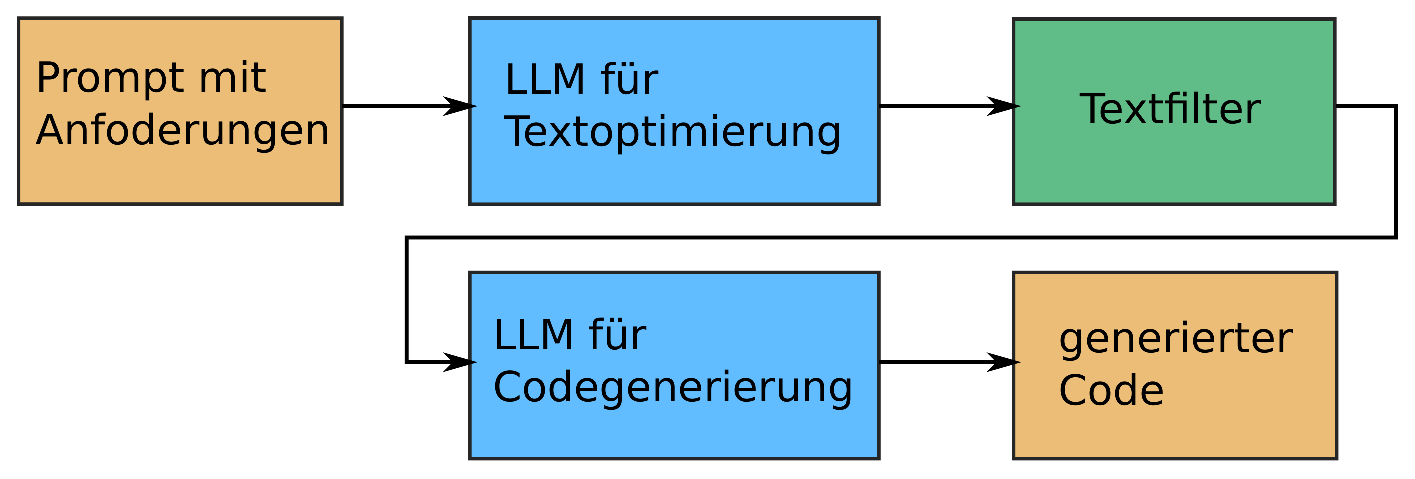
\includegraphics[width=0.8\textwidth]{content/chapter_implementation/images/orchestrierung_llms.eps}
%	\centering
%	\caption{Orchestrierte LLM's für die Codegenerierung}
%	\label{img:orchestration_llms}
%\end{figure}

%\section{Online Modelle}
%Text.

\subsection{Ergebnisse generieren}
Nachdem die Modelle bereitstehen, erfolgt das Generieren der Ergebnisse für jedes einzelne Modell. Mit Prompts, die aus den Proben des HumanEval-XL Benchmark bestehen, werden die Modelle mehrmals hintereinander abgefragt. Die vollständig generierten Antworten der Modelle werden, für eine spätere Auswertung und Nachvollziehbarkeit im \textit{JSONL}-Dateiformat gespeichert. Für jedes Problem erfolgen fünf Abfragen an jedes Modell. Welche Modelle für die Generierung verwendet wurden, ist in Kapitel \ref{subsec:llm_selection} nachzulesen. Alle Modelle wurde von Ollama-Framework bereitgestellt. Das Listing \ref{lst:python_generation_code} zeigt eine einfache Eingabeaufforderung, die an ein Modell gesandt wird.\vspace{0.2cm}

\begin{lstlisting}[
	language=Python,
	caption={Interaktion in Python mit Ollamaserver},
	label=lst:python_generation_code
]
from langchain_ollama.llms import OllamaLLM
from langchain.prompts import PromptTemplate

sample = read_sample_by(task_id=task_id)

model: OllamaLLM
answers: list = []
template = PromptTemplate(
    input_variables=["prompt"],
    template="{prompt}"
)
prompt = template.invoke({"user_prompt": sample.get("prompt")})

for index in range(0, 5):
    answers.append(model.invoke(prompt))

write_result(sample=sample.get("task_id"), answers=answers)
\end{lstlisting}

Nachdem die Proben in Zeile vier vom HumanEval-XL Benchmark eingelesen sind, wird in Zeile sechs bis zwölf das Modell und das Prompttemplate initialisiert. Um die Information \texttt{sample.get("prompt")} aus den Proben zu lesen, wird hier auf den Aufbau der Proben hingewiesen der in Kapitel \ref{subsec:structor_of_humaneval_xl} beschrieben wurde. Anschließend wird das Modell fünfmal abgefragt, hieraus lassen sich später, nach der \texttt{pass@k}-Methode, mit \texttt{k=\{0,...,5\}}, die Modelle evaluieren. Zum Schluss werden die Ergebnisse wie in Zeile siebzehn gezeigt, in JSONL-Dateien abgespeichert.

%---------------------------------------------------------------------------------------------------


\section{Optimierung der Antworten durch Änderung des Frameworks}
Wie das \texttt{langchain} Framework basiert das \texttt{DSPy} ebenfalls auf Python und eignet sich für die Abfrage lokale Ollama Modelle. Somit kann der vorhandene Ollama-Server genutzt werden.
Das Listing \ref{lst:python_generation_code_with_dspy} zeigt die einfache Initialisierung einer Interaktion mit einem lokalen Ollama Models mithilfe der \texttt{DSPy} Bibliothek.\vspace{0.2cm}

\begin{lstlisting}[
	language=Python,
	caption={Interaktion in Python mit Ollamaserver},
	label=lst:python_generation_code_with_dspy
]
import dspy

class BasicProgramming(dspy.Signature):
    question = dspy.InputField(desc="Eine Frage zu PHP Programmierung")
    answer = dspy.OutputField(desc="Generiere Programmcode")

model: dspy.LM = dspy.LM(
    api_base="http://192.168.1.56:11434", # required
    model="ollama_chat/deepseek-r1:32b", # required
    api_key="", # required
    temperature=0.2, # optinal
    cache=False, # optinal
    cache_in_memory=False, # optinal
)

dspy.configure(lm=model)
model(messages=[
    {
        "role": "user",
        "content": "Du bist erfahrener PHP Entwickler",
    }
])

chain = dspy.ChainOfThought(BasicProgramming)
\end{lstlisting}

Der Code zeigt Nach dem Bibliotheksimport wird die Signatur für die Abfrage erstellt. Hier wird die Interaktion mit dem Modell definiert. Es wird die erwartete Eingabe (\texttt{question}) und Ausgabe (\texttt{answer}) festgelegt. Die \texttt{desc}-Parameter im \texttt{InputField} und \texttt{OutputField} dienen lediglich für eine Beschreibung der Felder und haben keinen Einfluss auf den generierten Code.\vspace{0.2cm}

Im Anschluss wird das Lokale Modell mit erforderlichen und optionalen Parametern konfiguriert. Die Parameter \texttt{api\_base}, \texttt{model} und \texttt{api\_key} sind erforderlich. Wobei der Wert für \texttt{key} leer bleibt, solang der Ollama-Server keine Keys für die Anmeldung verwendet. Der Zusatz \texttt{ollama\_chat} veranlasst das Modell-Objekt nach einem Ollama-Server unter der, in \texttt{api\_base} angegebenen IP zu suchen. Mit einer \texttt{temperature}-Angabe von \texttt{0.2} wird das Modell zu einer deterministischen Antwort geleitet. Hier ist eine hohe Kreativität nicht gewünscht. Werden die optionalen Parameter \texttt{cache} und \texttt{cache\_in\_memory} nicht gesetzt, so wird ein Cache eingesetzt, was dazu führt, dass die Abfrage nur einmal in die LLM leitet und die Antwort in einem Cache abgelegt wird. Bei allen weiteren Anfragen würde diese Antwort wiederholt zurückliefert. Das würde bedeuten, das immer nur der $pass@k$ für $k=1$ erstellt werden könnte. Um dies zu verhindern, müssen beide Parameter den Wert \texttt{False} erhalten.\vspace{0.2cm}

Nachdem das Modell konfiguriert ist, wird in Zeile 16 DSPy mit dem Modell \texttt{model} konfiguriert und definiert somit deren Verwendung. Ab der Zeile 17 wird dann die Systemnachricht initialisiert. Diese Systemnachricht wird als erste Nachricht an die LLMs gesendet und legt dadurch den Kontext fest.\vspace{0.2cm}

Die letzte Zeile des Listings \ref{lst:python_generation_code_with_dspy} zeigt die Erstellung einer \texttt{ChainOfThought} Instanz mit der zuvor erstellten Signatur.


\subsection{Ergebnisse generieren}
\begin{tcolorbox}[
	enhanced,
	colback=red!5!white,
	colframe=red!75!black!50,
	title= Mein roter Faden
	]
	Mögliche Optimierungsstrategien
	\begin{itemize}
		\item mit dem Model Programming (DSPY) Ansatz: Python Bibliothek vorhanden \href{https://pypi.org/project/dspy/}{pypi.org | DSPy}.
	\end{itemize}
\end{tcolorbox}

%---------------------------------------------------------------------------------------------------


%\subsection{Auswertung der Modellantworten}
\section{Benchmark Codeevaluation}\label{sec:benchmark_evaluation}
Die Analyse der generierten Antworten muss für jedes Modell individuell angepasst werden, da die erzeugten Codefragmente zwischen den Modellen variieren. Insbesondere unterscheiden sich die Formate, in denen die Codesnippets generiert werden, beispielsweise durch \texttt{```php} oder \texttt{```php \textbackslash n <?php}. Dementsprechend erfordert die Extraktion des relevanten Codes aus den Modellantworten eine flexible Methode, die an das jeweilige Ausgabeformat der Modelle angepasst wird. Ein exemplarischer Lösungsansatz zur Extraktion des generierten Codes ist in Listing \ref{lst:code_extraction} dargestellt.\vspace{0.2cm}

\begin{lstlisting}[
	language=Python,
	caption={Codesnippet zur Extrahierung des Codes aus der LLM Antwort},
	label=lst:code_extraction
]
def get_generatet_code(code=code):
    if len(code.split("```php")) > 1: # find start
        code = code.split("```php")[1]
        code = code.split("```")[0]

    if code.startswith("<?php"): # find start
        code = code.split("<?php")[1]
        code = code.split("?>")[0]

    if len(code.split(r"\n}\n")) > 0: # find end
        code = code.split(r"\n}\n")[0] + "\n}\n"

    return code
\end{lstlisting}

Um den generierten Code zu evaluieren, wird dieser zusammen mit dem Test, der jeweiligen Probe aus dem Benchmark zusammengeführt. Das Ergebnis ist ein ausführbarer Code, der die geforderte Methode enthält. Mittels Python wird der Code getestet, ob der dieser ausführbar ist. Entsteht bei der Ausführung ein Laufzeitfehler erfolgt der Abbruch des Tests. Dieser kann ausgelöst werden durch eine nicht korrekte Syntax, einer Endlosschleife oder wenn die geforderte Methode nicht generiert wurde. All diese Ereignisse führen dazu, das die Probe als nicht bestanden gilt. Das Listing \ref{lst:php_interpreter_in_python} zeigt den Ausschnitt im Code zur Ausführung des PHP Interpreters in Python.\vspace{0.2cm}

\begin{lstlisting}[
language=Python,
caption={Codesnippet zur Ausführung des PHP Interpreters},
label=lst:php_interpreter_in_python
]
import subprocess

def test_answer(task_id, repetition):
    # read generated code
    answer = read_answer(task_id=task_id, repetition=repetition)
    answer = get_generatet_code(code=answer)

    # read test in HumanEval-XL
    test = read_sample(task_id=task_id).get("test")

    try:
        result = subprocess.run(
            ["php", "-r", f"{test}{answer}"],
            capture_output=True,
            text=True,
            check=False,
            timeout=5,
        )
    except subprocess.TimeoutExpired:
        return False

    if result.stderr.strip() == "":
        return True

    return False
\end{lstlisting}

Nachdem eine von fünf Antworten des Modells und der Test aus dem Benchmark vorliegen, erfolgt die Prüfung des generierten Codes. Diese wird im Listing \ref{lst:php_interpreter_in_python} ab Zeile zwölf gezeigt. Die Funktion liefert \texttt{True} zurück, wenn es keine Fehler im Test gab, sonst immer \texttt{False}. Das Exception-Handling ab Zeile 19 wird aufgerufen, wenn die PHP Ausführung in einer Schleife hängt. Hier wird ein \texttt{Timeout} abgefangen und somit gibt der Test als nicht bestanden. Aus den erhaltenen Ergebnissen, der Proben eines Tasks, berechnet die \texttt{pass@k} Methode, die \glqq Wahrscheinlichkeit das in \texttt{k}-Proben, eine korrekte Probe ist\grqq \, hinsichtlich Codegenerierung. Anschließend wird der Durchschnitt für die Zuverlässigkeit des Modells errechnet.\vspace{0.2cm}

\textbf{Umsetzung der pass@k Metric}\vspace{0.2cm}

Nach Abschluss der Tests werden die Ergebnisse mithilfe der \textit{pass@k}-Methode analysiert. In Python steht hierfür, die Bibliothek \textit{pass\_at\_k} zur Verfügung. Das Listing \ref{lst:custom_pass_at_k} zeigt die Implementierung der Methode gemäß Gleichung \ref{equ:pass_qt_k_complex} in Kapitel \ref{subsec:pass_at_k}, wie sie auch in der Python-Bibliothek verwendet wird.  


\begin{lstlisting}[
	language=Python,
	label=lst:custom_pass_at_k,
	caption={Berechnung der pass@k Metrik in Python}
]
def custom_pass_at_k(n: int, c: int, k: int) -> float:
    """
    :param n (int): numbers of total samples.
    :param c (int): number of currect samples.
    :param k (int): number of consider samples.
    """
    if n - c < k:
        return 1.0
    return 1.0 - np.prod(1.0 - k / np.arange(n - c + 1, n + 1))
\end{lstlisting}

%Die \textit{pass@k}-Methode dient zur Berechnung der Wahrscheinlichkeit, dass in $k$ Abfragen mindestens eine korrekte Lösung enthalten ist. Dazu
Die Methode erwartet drei Parameter. Der Parameter $n$ bezeichnet die Gesamtanzahl der Abfragen pro Probe. Der Parameter $c$ gibt die Anzahl der korrekten Abfragen innerhalb einer Probe an. Schließlich legt der Parameter $k$ fest, wie viele der besten Abfragen für die Bewertung berücksichtigt werden. Alle drei Parameter sind ganzzahlig (\texttt{Integer}), während das Ergebnis als Gleitkommazahl (\texttt{Float}) zurückgegeben wird.  

In dieser Arbeit werden die Werte $k=1$ und $k=5$ für die Evaluierung herangezogen. Nachdem jede Probe des HumanEval-XL-Benchmarks einzeln bewertet wurde, wird eine aggregierte Bewertung für das gesamte Modell ermittelt. Diese Berechnung erfolgt gemäß Gleichung \ref{equ:probability_of_success_per_model} in Kapitel \ref{subsec:pass_at_k}.  

% --- More Tests -----------------------------------------------------------------------------------


%\section{Codeevaluation mit Frameworks}
%Neben der bekannten Evaluationsmethode mit dem HumanEval Benchmark, wird hier eine weitere Testmethodik überprüft, die mit verschiedenen Validierungstools der jeweiligen Programmiersprache ausgeführt wird. Für die Erstellung der Abfragen wird das Python-Skript verwendet, was schon im Kapitel \ref{sec:benchmark_evaluation} vorgestellt wurde.

%\subsection{PHP Codeevaluation}
%Der Test wird bei den erweiterten Problemen durchgeführt und beginnt mit den Unit-Tests die mit \textit{PHPUnit} durchgeführt werden. Im Anschluss wird \textit{PHPMetrics} ausgeführt. Hierbei wird geprüft, ob die Codekomplexität und Wartbarkeit überprüft. Die Ausführung der Tests wird mithilfe eines Python-Skripts durchgeführt. Es wird eine PHP Datei erstellt, die mit den Frameworks geprüft wird.

%\subsection{JavaScript Codeevaluation}
%Text.

%\section{Online Modelle}
% Eigenen KI Server \href{https://www.computerweekly.com/de/ratgeber/Einen-KI-Server-mit-Ollama-und-Open-WebUI-einrichte}{Computer Weekly}
% Orchestrierung mit Python \href{https://pypi.org/project/multillm/}{multillm-Projekt}
% LangChain Library \href{https://python.langchain.com/api_reference/ollama/chat_models/langchain_ollama.chat_models.ChatOllama.html}{Example}
% \href{https://pypi.org/project/langchain-ollama/}{Python lib langchain-ollama}
% YouTube \href{https://www.youtube.com/@AICodeKing}{AICodeKing}

\chapter{Evaluation}\label{chap:evaluation}
Die Evaluation der Ergebnisse erfolgt im ersten Schritt anhand des HumanEval-XL Benchmarks. Dieser Benchmark wird in \cite{peng-2024} vorgestellt und erweitert den HumanEval \cite{chen-2021}. Der HumanEval-Benchmark evaluiert nur Python während der HumanEval-XL weitere Programmiersprachen und in verschiedenen Landessprachen unterstützt, darunter auch die deutsche Sprache. Neben Python sind auch Prompts für PHP und JavaScript enthalten, welche für die Webentwicklung wichtig sind. Die Datensätze des HumanEval-XL sind unter \href{https://github.com/FloatAI/humaneval-xl}{https://github.com/FloatAI/humaneval-xl} einsehbar und bestehen jeweils aus 80 Tests. Für jedes Problem werden zehn Lösungsvorschläge generiert, die im Anschluss auf die Aspekte der Syntaktik und Semantik evaluiert werden.\vspace{0.2cm}

\sout{Diese Tests fordern LLM's auf kleine Problem zu lösen. Aus diesem Grund werden weitere Tests erstellt mit umfangreicheren Anforderungen aus dem Bereich der Webentwicklung. Zu jedem Problem wird eine Musterlösung und ein Unittest erstellt. Der Aufbau für diese Bereitstellung orientiert sich an dem Format aus dem HunamEval-Benchmark.}\vspace{0.2cm}

Ein Versuch größere und komplexere Probleme zu lösen, hatte nicht den erwarteten Erfolg. Es sind viele Iterationen notwendig, um ein funktionierendes Ergebnis zu erhalten. Im Laufe der Iterationen sind die Prompts für die Modelle immer größer geworden und haben viele Missverständnisse bei den Modellen erzeugt. So das eine Zerlegung in kleine Probleme sich als sinnvoller erwies.\vspace{0.2cm}

Des Weiteren ist die Bewertung der Coding-Standards der jeweiligen Programmiersprache vorgesehen. Für die Prüfung der Standards wird ein SonarQube-Server verwendet, der sowohl PHP als JavaScript unterstützt. Ebenfalls wird die Qualität des Codes evaluiert. Das Augenmerk liegt auf die Lesbarkeit, Effizienz und Wartbarkeit des generierten Codes.\vspace{0.2cm}

%Optional werden einige Tests von zusätzlichen Tools validiert, beispielsweise bei der Validierung von PHP Files sind es Tools wie phpunit\footnote{phpunit steht unter \href{https://github.com/sebastianbergmann/phpunit}{https://github.com/sebastianbergmann/phpunit} zum Download bereit.} und Code\_Sniffer\footnote{Code\_Sniffer steht unter \href{https://github.com/squizlabs/PHP_CodeSniffer}{https://github.com/squizlabs/PHP\_CodeSniffer} zum Download zur Verfügung.} für die Validierung von JavaScript findet das Framework Jasmin\footnote{\href{https://jasmine.github.io/}{https://jasmine.github.io}.} Anwendung.\vspace{0.2cm}


\section{Modellbewertung mit HumanEval Benchmark}
Für die Bewertung wird das Vorgehen gewählt, welches in \cite{chen-2021} und \cite{peng-2024} beschrieben ist. Die Tests werden exemplarisch, mit den für die Webentwicklung relevanten Sprachen PHP und JavaScript durchgeführt. Die Evaluierung der Modelle wird auf den Ebenen \glqq einfache Fragen\grqq \ und \glqq komplexe Aufgaben\grqq \ erfolgen. Die \glqq einfachen Fragen\grqq \ werden bereits durch den zuvor genannten Benchmarks abgedeckt, sodass der entwickelte Fragenkatalog sich auf die Ebenen mit den \glqq komplexen Aufgaben\grqq \ konzentriert.\vspace{0.2cm}

Aus Ergebnisse der Tests, wird mithilfe der $pass@k$-Metrik, die Zuverlässigkeit der jeweiligen Modelle berechnet. Dieser Wert gibt an, mit welcher Wahrscheinlichkeit mindestens eine richtige Lösung unter $k$ ausgewählten Vorschlägen vorhanden ist.\vspace{0.2cm}

Dabei ist $n$ die Gesamtanzahl der Versuche, $c$ die Anzahl der korrekten Lösungen unter den $n$ Versuchen und $k$ gibt die Anzahl der Lösungen an die betrachtet wurden. Für die Berechnung der $pass@k$ Metrik wird die Formal \ref{lst:pass_at_k} verwendet, welche in \cite{chen-2021} vorgeschlagen wird.\vspace{0.2cm}

Für alle Probleme wurden jeweils zehn Abfragen erstellt und bewertet. Welche Modelle getestet an der Evaluation beteiligt waren und welche Ergebnisse ermittelt wurden, wird in Tabelle \ref{tab:prompt_results_open_models} gezeigt.

\begin{table}[!ht]
	\begin{tabular}{|l|r|r|}
		\hline
		\textbf{Model} & \textbf{pass@1} & \textbf{pass@5} \\
		\hline
		Llama3.3 70b-q2      &     --- &      --- \\
		Llama3.2             &  0,0275 &   0,4114 \\
		Llama3.1 8b (T600)   &   0,045 &   0,5302 \\
		Llama3.1 8b (T1200)  &   0,045 &  0,53472 \\
		Llama3.1-claude      &  0,0325 & 0,508929 \\
%		llama3.1$^{Param}$   &     --- &      --- \\
		Gemini Flash 1.5     &   0,045 &   0,3866 \\
		Qwen 2.5-Coder 32b   & 0,01875 &    0,239 \\
		Mistral-small 22b    & 0,02125 &   0,3061 \\
		Deepseek-coder-v2    &  0,1075 &   0,5875 \\
		Codellama 13b        &     0,0 &    0,025 \\
%		\hline
%		\multicolumn{4}{|l|}{$^{Param}$: Anpassung der Parameter bei der Abfrage} \\
		\hline
	\end{tabular}
	\centering
	\label{tab:prompt_results_open_models}
	\caption{Ergebnisse der pass@k Methode}
\end{table}

Das Modell \texttt{codellama} wurde ebenfalls getestet, hat aber beim Generierung von den Lösungen der PHP Probleme nicht gut abgeschnitten. Viele der Anforderungen wurden in Python erstellt und viele Tests sind als nicht bestanden gewertet wurden. Aus diesem Grund wird es bei den weiteren Betrachtungen nicht mehr beachtet.\vspace{0.2cm}

Des Weiteren wurden eine Reihe von Llama-Modellen getestet, unter anderem einige verschiedene Llama3.1 Modelle. Bei dem \textit{Llama3.1 8b} wurden zwei verschiedene Versuche durchgeführt mit jeweils unterschiedlicher Tokenlängen. Anders als bei \textit{ChatGPT 3.5} und \textit{Gemini 1.5} können die kleineren Modelle schon mit geringerer Tokenlänge valide Antworten erzeugen. Die unterschiedliche Tockenlängen haben kaum einen Einfluss auf das Ergebnis. Hier liegt der Unterschied bei nicht mal einen Prozent.\vspace{0.2cm}

Ein Ansatz zur Promptoptimierung, wurde bei den Tests evaluiert. So wurde ein Llama3.1 Model mit den Systemprompts des \textit{Claude Sonnet 3.5} Modell von der Firma Anthroppic erstellt. Dieser Ansatz konnte mit dieser Evaluierung nicht bestätigt werden. Der Unterschied liegt hier bei plus einem Prozent bei der pass@1 und minus drei Prozent bei der pass@5 Evaluation. Mögliche Ursachen hierfür könnten in einer fehlerhaften Erstellung des Modells oder die Aufforderungen sind nicht kompatibel mit einem Llama3.1 Modell. Eine weitere Möglichkeit sind unzureichendes Wissen über die Architektur des Quellmodells oder fehlendes implizite Informationen im Zielmodell. Ebenso könnte die Unbrauchbarkeit der Systemprompts für Codegenerierung die Ursache sein. Warum es keinen signifikanten Unterschied gab, könnte nicht abschließen geklärt werden. Die Ergebnisse sind in Tabelle \ref{tab:prompt_results_open_models} und in der Abbildung \ref{img:pass_at_k_results_by_llm} zu sehen.\vspace{0.2cm}

Ein letztes Modell aus der Llama3 Reihe, das dem Benchmark unterzogen wurde, ist das \textit{Llama3.3 70b}. Auswertung liegt zurzeit noch nicht vor\vspace{0.2cm}

\begin{figure}[!ht]
	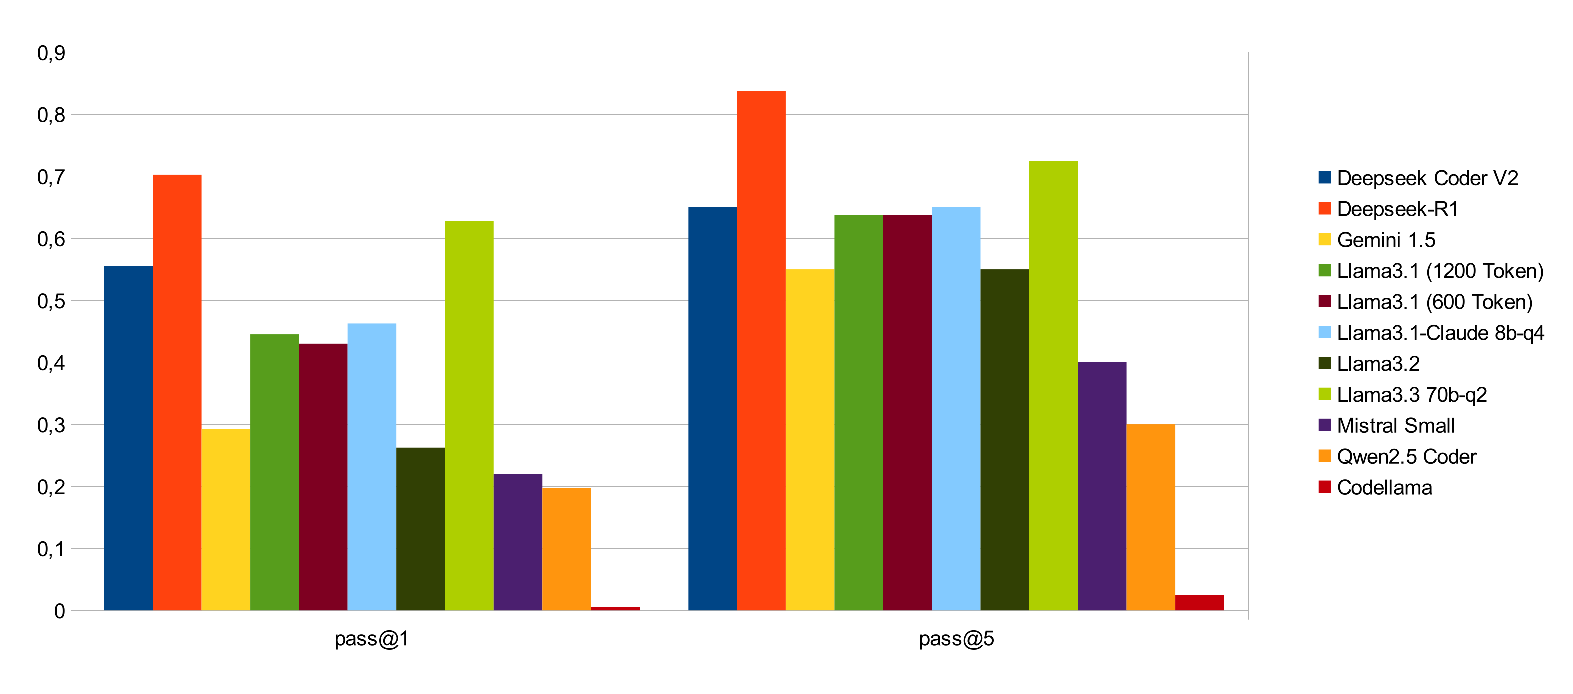
\includegraphics[width=\textwidth]{content/chapter_evaluation/images/llm_evaluation.eps}
	\centering
	\caption{Ergebnisse der pass@k-Methode für die Modelle}
	\label{img:pass_at_k_results_by_llm}
\end{figure}

Zwei weitere Modelle aus dem Open-Source-Bereich sind die Modelle \textit{Mistral-Small 22b} von der gleichnamigen Firma MistralAI und \textit{Qwen 2.5 Coder 32b}. Diese beiden Modelle schnitten im Vergleich nicht so gut ab. \vspace{0.2cm}

Das Modell \textit{Deepseek Coder V2 16b} welches an die Leistung von den Llama3.1 Modellen heranreicht.\vspace{0.2cm}
%Die Antworten von ChatGPT enthielten bei der ersten Abfrage Programmcode, alle weiteren Abfragen verwiesen auf den ersten Prompt. Eine Antwort ist in ?? dar gestellt, diese wurde in ähnlicher Weise immer wieder generiert.
%\hrulefill
%Der Code in deinem Kommentar ist identisch mit dem aktuellen Inhalt. Wenn du Än\-der\-ungen vornehmen möchtest, präzisiere bitte, was angepasst werden soll, und ich werde es umsetzen!
%\begin{flushright}
%	\textit{Generiert von ChatGPT 3.5}
%\end{flushright}
%\hrulefill

Ein weiteres Modell ist Gemini 15. von Google. Im Gegensatz zu den anderen Modellen, bringt Gemini nicht immer nur eine Lösung des Problems, sondern bietet weitere Ansätze, welche ebenfalls für das jeweilige Problem interessant sein könnten. Im folgenden Beispiel sind die verschiedenen Vorschläge des Modells in den Listings \ref{lst:gemini_result_php-3_1} bis \ref{lst:gemini_result_php-3_4} dargestellt, die beim PHP Problem 3 gefordert wurden. Die Aufgabenstellung in Kurzform war: \texttt{Gib den größten gemeinsamen Teiler von zwei ganzen Zahlen a und b zurück.}

\begin{lstlisting}[language=PHP,label=lst:gemini_result_php-3_1,caption={Gemini Ergebnis für das PHP-3 Problem Version 1}]
function greatestCommonDivisorRecursive($a, $b) {
  if ($b === 0) {
    return $a;
  } else {
    return greatestCommonDivisorRecursive($b, $a % $b);
  }
}
\end{lstlisting}

Neben den geforderten Lösung gab Gemini noch weitere Lösungsvorschläge aus. Das Listing \ref{lst:gemini_result_php-3_2} zeigt einen zweiten Lösungsansatz.\vspace{0.2cm}

\begin{lstlisting}[
	language=PHP,
	label=lst:gemini_result_php-3_2,
	caption={Gemini Ergebnisse für das PHP-3 Problem Version 2}
]
function greatestCommonDivisorBinary($a, b) {
  if ($a == 0) return $b;
  if ($b == 0) return $a;

  // Ensure a is odd
  if ($a % 2 == 0 && $b % 2 == 0)
    return 2 * greatestCommonDivisorBinary($a / 2, $b / 2);
  if ($a % 2 == 0) return greatestCommonDivisorBinary($a / 2, $b);
  if ($b % 2 == 0) return greatestCommonDivisorBinary($a, $b / 2);

  // a and b are odd
  if ($a > $b) return greatestCommonDivisorBinary($a - $b, b);
  return greatestCommonDivisorBinary($b - a, a);
}
\end{lstlisting}

Zu diesem Beispiel hat Gemini 1.5 noch weitere Lösungsansätze generiert. Diese sind in \ref{lst:gemini_result_php-3_3} und \ref{lst:gemini_result_php-3_4} zu sehen.

\begin{lstlisting}[
	language=PHP,
	label=lst:gemini_result_php-3_3,
	caption={Gemini Ergebnisse für das PHP-3 Problem Version 3}
]
function leastCommonMultiple(int $a, int $b): int {
  // kgV(a, b) = (a * b) / ggT(a, b)
  return abs($a * $b) / greatestCommonDivisor($a, $b);
}
\end{lstlisting}

\begin{lstlisting}[
	language=PHP,
	label=lst:gemini_result_php-3_4,
	caption={Gemini Ergebnisse für das PHP-3 Problem Version 4}
]
function greatestCommonDivisorMultiple(int ...$numbers): int {
  // ggT von mehreren Zahlen
  return array_reduce($numbers, 'greatestCommonDivisor');
}
\end{lstlisting}

Einige Aufgaben wurden von Gemini aber wie ein Chat behandelt. So hat das Modell Antworten generiert, die einer Konversation mit einem Chatbot ähneln, so wurde beispielsweise der folgende Text generiert, der einen Bezug zur zuvor gegebenen Antwort des Modells herstellt.

\hrulefill

\texttt{function greatestCommonDivisorRecursive(\$a, \$b) \{}

\texttt{\hspace{0.6cm} // ... (Rest der Funktion bleibt ähnlich)}

\texttt{\}}

\hrulefill

\begin{flushright}
	\textit{Generiert von Gemini 1.5}
\end{flushright}

Diese generierten Codeausschnitte haben die Tests nicht bestanden und wirken sich somit negativ auf die Auswertung aus.

\subsection{Nachteile der Evaluierung}
Es wird geprüft, ob der Code ohne Fehler ausführbar ist und die richtigen Ergebnisse liefert. Was dieser Test nicht evaluiert sind unter anderem vorhandene Codeerklärungen, Doc-Strings oder Code-Smells werden bei diesem Test nicht beachtet. Ebenso wird auch nicht der Codestandard geprüft.\vspace{0.2cm}

Benchmark prüfen, ob die Tests evtl. Fehler enthalten. Dies könnte sich beispielsweise in folgenden Probleme darstellen,

\begin{itemize}
	\item Tests sind falsch formuliert und die Abdeckung der geforderten Aufgabe wird nicht erfüllt, wodurch fehlerhafter generierter Code als korrekt bewertet wird.
	\item Fehler in den Musterlösungen können dazu führen, dass korrekte Lösungen als nicht bestanden gewertet werden.
	\item Mehrdeutige Aufgabenstellungen können ebenfalls das Ergebnis der Modelle negativ beeinflussen.
	\item Die Benchmark existieren bereit mehrere Jahre, sodass nicht ausgeschlossen werden kann, das Modelle explizit mit diesen Benchmarks trainiert wurden.
\end{itemize}

%--- Optimierung --------------------------------------------------------------------------------


\section{Optimierung der Ergebnisse}
Als Ziel der Optimierung gilt das die LLMs effizienten, präzisen und korrekten Code zu generieren. Ein Ansatz dies zu erreichen ist die Prompts zur Codegenerierung mithilfe einer LLMs zu erstellen oder zu verbessern.


% https://ki-techlab.de/ki-news/evaluierung-grosser-sprachmodelle-ein-technischer-leitfaden/

%\begin{tcolorbox}[
%	enhanced,
%	colback=BhtColorYellow!5!white,
%	colframe=BhtColorYellow!75!black,
%	title= HTML Startseite
%	]
%	Text in der Box
%\end{tcolorbox}

%\begin{tcolorbox}[
%	enhanced,
%	colback=BhtGrey!5!white,
%	colframe=BhtGrey!75!black!50,
%	title= ChatGPT 3.5
%	]
% Text in der Box
%\end{tcolorbox}


\chapter{Lessons Learned}\label{chap:lessons_learned}
In diesem Kapitel werden die Arbeitsprozesse der Evaluation und Optimierung reflektiert. Des Weiteren werden Vorschläge gegeben, um das Arbeiten mit Sprachmodellen zu verbessern.\vspace{0.2cm}

Zudem werden die größten Hindernisse und Probleme besprochen, die während der es gesamten Prozesses Evaluation auftraten. Diese beinhalten die Bereitstellung er Modelle, das Erheben der Daten zu den Proben des Benchmarks und deren Auswertung. Um in folgenden Arbeiten diese Fehler zu verhindern werden dazu Lösungsansätze und Vorschläge diskutiert.

% --- Evaluierung ----------------------------------------------------------------------------------


\section{Evaluierungsaufbau und Vorbereitung}
Um die Evaluierungen an Open-Source-Modellen durchführen zu können, mussten diese lokal bereitgestellt werden. Die Wahl viel auf das Ollama-Framework, da die Installation und Konfiguration sehr gut durch den Hersteller und verschiedene Foren unterstützt wird. Neben der vorhandenen API kann das Tool Open-WebUI einfach in das Ollama-Frameowrk integriert werden. Diese UI bietet eine gute UI die von allen Clients im Netzwerk aufgerufen werden kann. Ebenfalls ein großer Vorteil sind die vielen Modelle welche für Ollama zum Download bereitstehen. Darunter sind Modelle von Mistral, Llama, Deepseek und Qwen-Coder.\vspace{0.2cm}

Eine weitere Möglichkeit ist, die Modelle lokal auszuführen ohne ein Framework einzusetzen. Hierbei können die Abfragen nur auf dem lokalen System erfolgen, wenn keine eigene API Schnittstelle erstellt wird. Unter anderem war keine Web-UI vorhanden, sodass diese Möglichkeit nicht weiter in Betracht gezogen wurde.\vspace{0.2cm}

%---------------------------------------------------------------------------------------------------


\section{Evaluierung der großen Sprachmodelle}
Ein großes Problem stellte der Zugriff auf die Cloused-Source-Modelle dar. Durch die beschränkten Bezahlmethoden konnte ein permanenter Zugriff auf die Modelle nicht erfolgen. Aus diesem Grund wurden hauptsächlich Open-Source-Modelle lokal evaluiert und getestet.


\subsection{Lokale Ressourcen}
Eines der größten Probleme für das lokale Betreiben von großen Sprachmodellen sind die Hardwareanforderungen. Hier spielen neben der Prozessoranzahl, die Speicherplatz der Festplatte und der VRAM der Grafikkarte eine Rolle. Während der Arbeit wurde eine SSD-Festplatte mit höherer Kapazität eingesetzt und eine Grafikkarte mit mehr VRAM.\vspace{0.2cm}

Der größere Speicher wurde notwendig während des Laden und Speichern der Modelle auf die lokale SSD. Zudem war ein RAM notwendig, der doppelt so groß sein musste wie das Modell selbst. Um diesen RAM bereit zustellen wurde eine SWAP Partition von 100 GB auf der SSD eingerichtet. Dieser wurde auch für die Ausführung größerer Modelle benötigt.\vspace{0.2cm}

Eine weitere Verbesserung war der Austausch der Grafikkarte. Hierbei wurde die vorhandene Nvidia GTX 1050 TI mit 4 GB VRAM und einer Bandbreite von 112 GB/s durch eine Nvidia RTX 3060 mit 12 GB VRAM und einer Bandbreite von 360 GB/s ersetzt. Durch das Austauschen der Grafikkarte wurde der SWAP für die Berechnungen der Token während die Antwort erstellt wurde nicht mehr benötigt.

Durch diese Anpassungen bestand die Möglichkeit größere Modelle zuladen und bereit zustellt. Des Weiteren konnte eine wesentliche Verbesserung der Antwortzeit festgestellt werden. Eine genaue Messung wurde hier nicht durchgeführt. So wurden bei dem Deekseek-Coder-V2 Modelle eine Verbesserung der Berechnungszeit für den Benchmark von etwa 24 Stunden auf circa eine Stunde beobachtet.\vspace{0.2cm}

Dennoch war die Berechnungszeit einiger Modelle, welche mehr als 12 GB groß waren sehr hoch. Sodass die Wartezeit, das Auswerten der Evaluierung verzögerte.


\subsection{Auswertung des Benchmarks}
Die Anwendung des vorgeschlagenen Parametersatzes zeigte bemerkenswerte unerwünschte Auswirkungen auf die Erzeugung der Antworten. Insbesondere bei einer Tokenlänge von 600 traten Störungen auf, die den generierten Codeabschnitt entweder gänzlich oder nur teilweise verfügbar machten. Diese Ungenauigkeit resultierte beim \textit{DeepSeek-R1} aus einem 'explanation'-Abschnitt innerhalb der Antwortstruktur, in dem das Modell eine detaillierte Herleitung seines Denkprozesses anbot, bevor es zur eigentlichen Lösung gelangte. Bei den Modellen \textit{ChatGPT 4} und \textit{Gemini 1.5} führten ausführliche Erklärungen am Anfang und am Ende der Antwort zum selben Effekt, sodass diese Ergebnisse ebenfalls nicht brauchbar waren. Aus diesem Grund wurde beim \textit{DeepSeek-R1} und beim \textit{Gemini 1.5} auf eine Einschränkung der Tokenlänge verzichtet. Auf eine erneute Evaluierung des OpenAI Modell müsste aus Kostengründen verzichtet werden.\vspace{0.2cm}

Bei der Auswertung des Benchmarks traten einige Fehler auf, die beseitigt werden konnten. Ein Großteil waren kleinere Fehler, die bei der Auswertung aufgetreten, wie in Kapitel \ref{subsec:disadvantages_of_evaluation} bereits angesprochen. Der gravierendste Fehler trat aber bei der Berechnung das \texttt{pass@k} für das gesamte Modell auf. Hier wurde eine falsche Python-Methode implementiert, sodass das Ergebnis, um ein Vielfaches niedriger war, als das wirkliche Ergebnis. Erst durch den Vergleich mit Ergebnisse anderer Arbeiten und den Herstellerangaben ist der Fehler aufgefallen. Nach intensiver Suche wurde dieser gefunden und beseitigt.\vspace{0.2cm}

Bewehrt hat sich hier der Einsatz von Python und dessen Bibliotheken für Umsetzung der Evaluierungsaufgaben. Mittlerweile existieren für die meisten Probleme und Anforderungen bereits fertige Bibliotheken oft von den Herstellern der Modelle selbst. Basierend auf den vorhandenen Bibliotheken, konnte die Entwicklung der Evaluationsaufgaben in kurzer Zeit umgesetzt und implementiert werden.\vspace{0.2cm}

% --- Evalierung mit eigenen ---------------------------------

\begin{tcolorbox}[
	enhanced,
	colback=red!5!white,
	colframe=red!75!black!50,
	title= Mein roter Faden
	]
	Hier folgen noch die Ergebnisse zur Optimierung.
\end{tcolorbox}

% --- Optimierung ----------------------------------------------------------------------------------


\section{Optimierung der Abfragen}


\subsection{Erweiterte Codeevaluation}
Bei den vordefinierten Prüfungen der HumanEval Benchmarks, wird geprüft, ob der Code lauffähig ist, nicht aber die Codestruktur oder Kommentare. Ein Problem bei der Nutzung des von der LLM generiertem Code ist, dass Entwickler diesen einfach kopieren und in ihre Programme implementieren. Es wird also nur die Funktionalität des Codes geprüft, nicht aber Strukturen und Kommentare um die Lesbarkeit und Verständlichkeit zu erhöhen. Dieses Vorgehen mag zu schnellen Erfolgen in der Programmentwicklung führen, wird aber beim Refactoring oder Fehlersuche erhebliche Defizite mit sich bringen.\vspace{0.2cm}

Aus diesem Grund sollte der erstellte Code nicht nur auf die Funktionalität geprüft werden. Dafür sollten weitere Test-Frameworks der jeweiligen Programmiersprache zur Anwendung kommen. Es gibt mehrere Frameworks zur Prüfung der Codequalität unter PHP. Zwei bekannte Frameworks die auch in dieser Arbeit Anwendung finden, sind die Frameworks \texttt{phpunit} und \texttt{phpmetrics}. Mit ihnen wird der, durch die LLMs generierten Codes geprüft.\vspace{0.2cm}
Um PHPUnit und PHPMetrics für die Evaluierung zu verwenden, müssen weitere Angaben und Einträge im Benchmark erfolgen. So muss ein PHP-Unittest enthalten sein, dieser kann den einfachen benutzerdefinierten Test ersetzen. Des Weiteren sind die Kriterien für die Metrik Messung, für jeden Test erforderlich. Die Kriterien können wie in Listing \ref{lst:phpmetric_criteria_example} dargestellt, aussehen.

\begin{lstlisting}[language=python,caption={Beispiel für Bewertungskriterien},label=lst:phpmetric_criteria_example]
	criteria = {
		"Lines of code": lambda x: int(x) > 12,
		"Logical lines of code by method": lambda x: float(x) > 7,
		"Lack of cohesion of methods": lambda x: float(x) > 3,
		"Average Cyclomatic complexity by class": lambda x: float(x) > 10,
		"Average Weighted method count by class": lambda x: float(x) > 20,
		"Average bugs by class": lambda x: float(x) > 0.1,
		"Critical": lambda x: int(x) > 0,
		"Error": lambda x: int(x) > 0,
		"Warning": lambda x: int(x) > 0,
		"Information": lambda x: int(x) > 0,
	}
\end{lstlisting}

Mit den erweiterten Tests werden die Benchmarks, um die folgenden Punkte erweitert.

\begin{myitemize}
	\item \textbf{unittest}: Unittests für die geforderte Funktion, unterschied zu den einfachen Tests
	\item \textbf{metrics}: Kriterien für den Metriktest
\end{myitemize}

\subsection{PHPUnit}
Eines der bekanntesten spezielles Framework für Unit-Tests in PHP, was als Industriestandard gilt. Mit diesem Framework können neben der Prüfung auf funktionsfähigen Code auch Randfälle betrachtet und Fehlerbehandlungen im Code getestet werden. Als Grundlage für die Auswahl des Tools wird auf Studie \cite{mohamad-2016} verwiesen.

\subsection{PHPMetrics}
Ein PHP Framework für die Codeanalyse, welches detaillierte Berichte über die Codequalität, Komplexität des Codes und über dessen Wartbarkeit erzeugt. PHPMetrics wird in verschiedenen Arbeiten eingesetzt, um die Codequalität zu ermitteln. So auch in \cite{anggrain-2016}, bei der verschiedene Open Source LMS verglichen werden.

%\subsection{SonarQube}
%Als letztes Tool soll SonarQube zur statischen Codeanalyse und Codeprüfung zum Einsatz kommen. Es werden verschiedene Programmiersprachen unterstützt, darunter auch PHP und JavaScript. In der Arbeit \cite{da-silva-simoes-2024} wird die Prüfung der Codequalität mit SonarQube, ChatGPT3.5 und ChatGPT4 vergleichen. Als Schlussfolgerung aus dem Ergebnis dieser Arbeit, wird auch hier die Codeanalyse durch eine LLM nicht erfolgen, sondern ebenfalls durch SonarQube.

%\subsection{ESLint}
%JavaScript Tool zur Syntaxfehler-Erkennung, Stil- und Codequalitätsprüfung. Mit diesem Tool kann reines JavaScript als auch Node.js überprüfen. https://arxiv.org/html/2402.14261v1


\chapter{Diskussion und Ausblick}\label{chap:discussion}
\begin{tcolorbox}[
	enhanced,
	colback=red!5!white,
	colframe=red!75!black!50,
	title= Mein roter Faden
	]
	Struktur des Kapitels
	
	\begin{enumerate}
		\item \textbf{Einleitung}: Eine kurze Einführung in die Diskussion und den Ausblick.
		\item \textbf{Zusammenfassung der Ergebnisse}: Eine kurze Übersicht über die wichtigsten Ergebnisse und in Relation mit den Forschungsfragen stellen.
		\item \textbf{Diskussion der Ergebnisse}: Eine Analyse und Interpretation der Ergebnisse. Vergleich mit Stand der Forschung und früherer Arbeiten.
		\item \textbf{Grenzen und Einschränkungen}: Eine Diskussion der Limitationen der Studie. Z.B. begrenzte Datenbasis, Grenzen der eingesetzter Tools und Technik.
		\item \textbf{Impulse für zukünftige Forschung}: Vorschläge für weitere Studien. Verbesserungsmöglichkeiten der Methoden usw. und Zukunft des Forschungsfeldes und evtl. Trends.
		\item \textbf{Praktische Anwendung}: Eine Diskussion der möglichen Anwendungen der Ergebnisse. In welchen Unternehmen und welche realen Anwendungen können die Ergebnisse eingesetzt werden.
	\end{enumerate}
\end{tcolorbox}

Dieses Kapitel stellt eine Zusammenfassung der wichtigsten Ergebnisse dieser Arbeit auf, die zur Beantwortung der Thesen führen. Es werden zusammenfassend die Grenzen und Einschränkungen geklärt, zu denen die Evaluation durchgeführt wurde. Des Weiteren werden Impulse für weitere Forschungen diskutiert. Das Kapitel endet mit einer praktischen Anwendung, bei der die Ergebnisse dieser Arbeit angewandt werden können.

%Vergleich Stand der Forschung: fehlt noch, muss in Thesen einfließen

\section{Bewertung der Zielsetzung und Thesen}
% 3. These: Optimierung ohne Modellanpassung, nur Prompt Engineering
Die Erkenntnisse aus den Experimenten dieser Arbeit bestätigen die aufgestellte dritte These (T3) aus Kapitel \ref{sec:goals_of_the_work}. Eine Optimierung der Eingabeaufforderungen für die Webanwendungsentwicklung lässt sich ohne Änderung der Modellparameter erreichen und bewirken eine signifikante Verbesserung der Ergebnisse. Die Modelle wurden bereits mit Programmiersprachen, die für Webanwendungsentwicklung essenziell sind, wie beispielsweise PHP, trainiert und diese Daten, in Form von Programmcode sind in den Modellen abrufbar. Entscheidend hierbei ist die Art und Weise wie die Gestaltung der Eingabeaufforderungen umgesetzt wird. Diese Optimierung erfolgt durch das \texttt{DSPy} Framework für die meisten Modelle automatisch.\vspace{0.2cm}

% Hat nicht funktioniert.
Dennoch hat das \texttt{DSPy} Framework, auf einige Modelle eine negative Auswirkung. Der generierte Code schnitt in der Evaluation mit den HumanEval-XL Proben schlechter ab. Der Grund konnte zurzeit nicht geklärt werden. Eine Annahme ist, dass der deklarative Ansatz von DSPy mit den komplexeren Datenstrukturen und Modulketten die LLMs zu inkonsistenten Antworten leitet. In diesen Fällen sollte weitere Frameworks, wie beispielsweise \textit{AdalFlow} oder \textit{LamaIndex} für die Optimierung in Betracht gezogen werden.\vspace{0.2cm}

% Es gibt Fehler bei der Verwendung von DSPy.
Die Tests haben weiterhin gezeigt, dass einige Modelle nicht mit dem \texttt{DSPy} Framework zusammenarbeiten. Auch hier konnte nicht abschließend geklärt werden, ob die Fehlerquelle bei der eingesetzten Hardware zu suchen ist oder ob das Framework selbst Probleme mit den Antworten dieser Modelle hat. Bei Modellen, die dieses Verhalten zeigen, sollte geprüft werden, ob auch hier die Wahl auf ein anderes Framework fallen kann.\vspace{0.2cm}

Gerade mit der Arbeit von Closed-Source-Modellen, bei der die Modelle gar nicht oder nur sehr bedingt angepasst werden können, sind die Optimierungen der Eingabeaufforderungen essenziell.\vspace{0.2cm}

% 2. These: Benckmarks sind ungeeignet
Alle Evaluierungen wurden mit den HumanEval-XL durchgeführt. Mit den gewonnenen Erkenntnissen aus dieser Arbeit lässt sich die zweite These (T2) nur bedingt bestätigen. Ein einzelner Benchmark hat nicht ausreichend Aussagekraft, um eine LLM hinreichend zu bewerten. Diese Benchmarks eignen sich um einen ersten Eindruck von den Modellen zu erhalten. Hierbei können erste Eindrücke über deren Stärken und Schwächen gesammelt werden. Wie auch in \cite{zhang-2024} wird die Auffassung vertreten, dass diese Probe grundlegende Codeproblematiken testen, die nicht mit den realen Anforderungen von Entwicklern übereinstimmen. In dem Onlineartikel \cite{albrecht-2023} heißt es \glqq \textit{...liefert Code, der zwar nicht immer direkt nutzbar ist, nach einer Überarbeitung aber schon recht überzeugend läuft.}\grqq. Diese Aussagen deuten darauf hin, dass Programmierer andere Anforderungen an LLMs stellen, die zurzeit mit Benchmarks nur in engen Grenzen abgedeckt werden können.
Die menschliche Intelligenz ist in der Lage aus generiertem Code und eigenem Wissen, die Programmteile herauszufiltern welche zur Lösung eines Problems beitragen. Entwickler stellen meist sehr komplexe Anforderungen, um die ihnen gestellten Probleme zu lösen. Diese Komplexität wird durch die Benchmarks nicht abgedeckt.\vspace{0.2cm}

% 1. These: LLMs effizientere Webanwendungsentwicklung. Wichtig ist die Evaluierung
In den letzten Jahren hat generative KI auch die Arbeit der Entwickler stark beeinflusst. So ist in \cite{focus-online-2025} die Rede von einem Programmierer, der seine Aufgabe abbrach, Zitat: \glqq \textit{weil er keinen Zugang zu seinem virtuellen Assistenten hatte. ''Ich kann einfach nicht mehr ohne die Hilfe der KI programmieren''}\grqq \ so der Entwickler. In \cite{company_gartner_2024}, einem Artikel von Gartner, wird behauptet das bis zum Jahr 2027, 80\% der Ingenieure eine Weiterbildung für generative KI benötigen. Dies hebt ebenfalls den Trend der nächsten Jahre hervor, das generative KI die Softwareentwicklung maßgeblich beeinflussen wird.
% Zu den Modellen.
Die Beliebtheit von KI Anwendungen wächst bei Softwareentwicklern immer weiter und dies gilt auch für den Bereich der Webanwendungsentwicklung. Dabei nutzen viele Entwickler, KI Modellen von US amerikanischen Unternehmen wie Athropic, Google oder OpenAI die bereits sehr gut entwickelte Chatbots und APIs anbieten, welche für die Integration in Tools zur Codegenerierung eingesetzt werden können. Zurzeit hat Mistral, eine europäische KI-Entwicklungsfirma einen neuen Chatbot, mit names \textit{Le Chat} herausgebracht, der Kokurrenz zu den amerikanischen Konzernen gesehen wird. Die KI-Entwicklungsfirma \textit{Deepseek} aus China hat ein Modell entwickelt, das wie Mistral in Konkurrenz zu den amerikanischen Modellen steht. Neben diese kommerziellen Closed-Source-Modelle gibt es eine Reihe von Open-Source-Modellen, welche ebenfalls hervorragende Resultate für die Generierung von Code zeigen, wie die Ergebnisse dieser Arbeit beweisen. Um so wichtiger ist es die Stärken und Schwächen der Modelle zu kennen und welche Methoden, zur effektiven Nutzung von Eingabeaufforderungen einzusetzen sind. Mit diesen Kenntnissen wird die, in der Arbeit aufgestellte dritte These (T3) bewiesen. Ki kann und wird die Webanwendungsentwicklung maßgeblich beeinflussen.\vspace{0.2cm}

Gerade die einfache und effiziente Suche mithilfe der LLMs bring einen zeitlichen Vorteil, dessen Ergebnisse bereits mit einfachen Tests überprüft werden können. LLMs reduzieren die Suche nach geeigneten Frameworks und Technologien und liefern fast immer funktionsfähigen Code. Dies gilt für die Integration in \acrshort{IDE} wie auch die Nutzung eines Chatbots.

\section{Grenzen und Einschränkungen}
%Kleine Beteiligung der Closed-Source-Modelle aufgrund der Kosten.
Die in dieser Arbeit evaluierten und optimierten Modelle, waren hauptsächlich Open-Source-Modelle. Alle diese Modelle wurden von der Plattform Ollama bereitgestellt. Zwei Ausnahmen gab es bei der Evaluierung, hierbei handelt es sich um \textit{Gemini 1.5} von Google und \textit{ChatGPT 4} von OpenAI.\vspace{0.2cm}

%Benchmark nur den HumanEval-XL, mit 80 Proben.
Für die Evaluierung der Modelle ist nur der \textit{HumanEval-XL} angewandt worden. Die meisten Benchmarks prüfen LLMs mit Python oder Java Proben. Eine Evaluierung mit spezifischen Sprachen für Webanwendungsentwicklung wie PHP, bieten nur wenige Benchmarks.\vspace{0.2cm}

%Nur langchain und DPSy
Die Auswahl der getesteten Frameworks, welche die Kommunikation zu den LLMs und somit zum Ollama-Server herstellten, waren begrenzt auf \texttt{langchain} und \texttt{DSPy}.\vspace{0.2cm}

\section{Impulse für zukünftige Forschungen}
%Ein interessantes Feld für die Forschung ist die Nutzung generativer KI und welche Auswirkungen dies auf das menschliche Denken und Handeln hat. In der Studie \cite{chiriatti-2024} wird von einem System 0 gesprochen, welches neben den bekannten 
%\begin{enumerate}
%	\item System 1: schnelles,intuitives und automatisches Denken
%	\item System 2: langsameres, analytisches und reflektierteres Denken
%\end{enumerate}

%eingeführt wird. Hierbei handelt es sich um ein Denken, welches die KI für den Menschen übernimmt. Entscheidungen und Daten werden durch die KI übernommen. Ein externes System, ähnlich wie eine USB-Festplatte eines PCs.\vspace{0.2cm}
% Immer neue Modelle
Die KI-Entwicklungsfirmen bringen immer neue Modelle auf dem Markt, die schon mit einer sehr kleinen Anzahl vom Parametern gute Ergebnisse liefern. Hier könnte eine Studie zeigen, ob \textit{Small Language Models} (SLM) mit den \textit{Large Language Models} (LLM), im Bereich der Webanwendungsentwicklung konkurrieren können. Ein Beispiel für ein SML ist das Modelle \textit{Phi} von Mirosoft, welches beispielsweise unter \cite{phi2_huggingface_2024} heruntergeladen werden kann. Wird ein Modell für die Codegenerierung eingesetzt und dahin gehend optimiert, ist die Menge an Parametern nicht erforderlich. Es existieren bereits einige Studien zu diesem Thema. Beispielsweise wird in \cite{hu-2024} eine allgemeine Verbesserung des Benutzererlebnisses untersucht und in \cite{irugalbandara-2023} wird eine Reduzierung der Kosten in Produktionsumgebungen vorgestellt.\vspace{0.2cm}
%Inwieweit können auch \textit{Small Language Models} für Programmieraufgaben eingesetzt werden. Könnte der enorme Energiebedarf und Ressourcen der LLMs durch SLMs ersetzt werden? Siehe \href{https://medium.com/@nageshmashette32/small-language-models-slms-305597c9edf2}{Small Language Models (SLMs)} oder \href{https://medium.com/version-1/small-but-powerful-a-deep-dive-into-small-language-models-slms-b793bdb002f2}{Small but Powerful: A Deep Dive into Small Language Models (SLMs)}. Eine weitere Forschung kann die Evaluation sein, ob Finetuned SLMs, wie Phi-2, Google Gemini Nano oder Metas Llama-2-13b bessere Ergebnisse liefern, als die LLMs.\vspace{0.2cm}

% Andere Benchmakrs eigene entwickeln.
Des Weiteren sollte Unternehmen oder Entwickler weitere Benchmarks in Betracht ziehen und die Brauchbarkeit von LLMs für die Webanwendungsentwicklung evaluieren. Interessant wäre die Prüfung, ob die Verwendung mehrerer Benchmarks zu einer besseren Bewertung der LLMs führt.\vspace{0.2cm}

Da die meisten Benchmarks auf statische Analysen ausgelegt sind und die LLMs nur bedingtes oder klein deterministisches Verhalten zeigen, kann eine weitere Forschung dahin gehen, einen Benchmark zu erstellen, der auf die dynamischen Antworten der LLMs besser eingehen könnte. Speziell für die PHP-Entwicklung wäre eine Untersuchung interessant, bei der die Evaluierung mit externer Tool wie \textit{SonarQube}, \textit{PHPBench}, \textit{PHPUnit} oder \textit{PHPMetrics} durchgeführt und dadurch eine verbesserte Bewertung der LLMs  erreicht wird.  Analog kann so ein Benchmark auf für andere relevante Programmiersprachen der Webentwicklung, wie beispielsweise JavaScript, Java und Ruby ausgeweitet werden.\vspace{0.2cm}

% Einführung in Firmen und Schluung der Mitarbeiter.
Ein weiteres mögliches Themenfeld ist die Einführung einer KI gestützten Softwareentwicklung für Webanwendungen mit Firmenrichtlinien. Der Fokus sollte hierbei auf das Auswahlverfahren der Modelle liegen mit Blick auf die möglichen Benchmarks und dem Evaluierungsverfahren. Wie lassen sich Entwickler frühzeitig in die Auswahl der Modelle einbeziehen und welche Möglichkeiten bestehen für Entwickler schon während dieses Prozesses ihre Kenntnisse im Bereich von generativer KI zu erweitern oder vertiefen, sodass effektives Entwickeln von Anfang an erfolgen kann.\vspace{0.2cm}
%\begin{tcolorbox}[
%	enhanced,
%	breakable,
%	colback=red!5!white,
%	colframe=red!75!black!50,
%	title= Mein roter Faden: noch was zum Testen
%	]
%	Ein Tool zur Orchestrierung von Multi-Agenten-Systemen \href{https://community.openai.com/t/introducing-swarm-js-node-js-implementation-of-openai-swarm/977510}{OpenAI Swarm}, gefunden auf \href{https://karrierewelt.golem.de/blogs/karriere-ratgeber/bot-belegschaft-mit-entlastungspotenzial-ki-agenten-fur-den-arbeitsalltag-in-der-testphase-1}{Golem | Karrierrewelt}.
%\end{tcolorbox}

\section{Praktische Anwendung}
%Praktische Anwendung: Eine Diskussion der möglichen Anwendungen der Ergebnisse. In welchen Unternehmen und welche realen Anwendungen können die Ergebnisse eingesetzt werden.
% Konkreter Fall
In der kommenden Zeit wird die Entwicklung der LLM weiter voranschreiten, dies wird zu weiteren Verbesserungen bei den Ausgaben der LLMs führen. Dennoch sollte der Focus auf eine einheitliche Vorgehensweise liegen. Somit werden nicht nur gleiche Standards beim Code geschaffen, zudem wird ein einheitliches Know-How der Mitarbeiter realisiert. Dies wird langfristig dazu führen, dass die Entwicklung von Webanwendungen mithilfe generativer KI, die Arbeit der Entwickler effizienter gestaltet und sich somit auf die Kosten und Ressourcen der Unternehmen auswirkt.\vspace{0.2cm}

% Nutzen/Vorteil
Die Auswahl der Anbieter wird, durch deren ständig wachsender Anzahl immer schwieriger. Die in dieser Arbeit evaluierten Modelle, können Unternehmen nutzen, um einen Einstieg in das Thema zubekommen und schlägt Modelle vor, welche sich für die Generierung von Programmcode in der Webanwendungsentwicklung eigenen. Des Weiteren unterstützt diese Arbeit sie den bei ersten Versuchen, weitere neue LLMs zu evaluieren und das optimale Modell für ihre Prozesse zu finden. Die Mehrheit der Entwickler und Unternehmen nutzt zurzeit kommerzielle Modelle großer Anbieter, da die Nutzung der Chatbots und schnelle, unkomplizierte Verwendung der APIs mit wenig Aufwand realisierbar ist. Durch das zunehmende breite Interesse an generativer KI, wurden Möglichkeiten geschaffen Open-Source-Modelle in der eigenen Infrastruktur einzubinden und diese zu verwenden. Dies kann, wie schon zuvor besprochen zur Senkung der Kosten beitragen. Besonders die Abrechnung der Tokens ist ein interessanter Punkt, der nicht immer eindeutig nachvollziehbar ist. Der Kostenaspekt zwischen \textit{Open-Source} und \textit{Closed-Source} Modellen, wurde schon aufgegriffen, diskutiert und bringt laut \cite{irugalbandara-2023} eine große Ersparnis, was nicht nur für kleine und mittlere Unternehmen interessant werden kann. Wie in dieser Arbeit gezeigt, liefern die Open-Source-Modelle hervorragende Ergebnisse für die Aufgaben in der Webanwendungsentwicklung, oft bessere als die kommerziellen Closed-Source-Modelle.\vspace{0.2cm}

% Implementierung
Unabhängig von der Auswahl des Modells sollten Unternehmen für die Entwickler einheitliche Schnittstellen zu den Modellen bereitstellen. Zum Einem können die Eingabeaufforderungen, wie in dieser Arbeit beschrieben, mittels verschiedener Frameworks oder anderer Methoden angepasst werden. Zum anderen können die abgesetzten Prompts verwendet finden, um Modelle weiter, durch \glqq Fine-Tuning\grqq \ zu optimieren. Eine weitere Möglichkeit besteht darin die Prompts auszuwerten und den Wissensstand der Entwickler zu prüfen und ggf. mit gezielten Schulungsmaßnahmen das Entwicklungsteam zu fördern.\vspace{0.2cm}

Ein weiterer Vorteil dieser Methode ist, dass die Prompts mit verschiedenen Metadaten angereichert und Ansätze wie \textit{Personas}, \textit{Beispielen} und \textit{zusätzlichem Kontext} umgesetzt werden können. Vorstellbar wäre auch die Integration eines RAG, welches auf Daten der eigenen Entwickler und bereits umgesetzter Softwarelösungen zurückgreifen kann.\vspace{0.2cm}

% Example
Die Abbildung \ref{img:example_firm_integration} zeigt das zuvor beschriebene Beispiel für die Integration einer LLM in den Prozess zur Programmcodegenerierung. Die Entwickler stellen ihre Eingabeaufforderungen an den Agenten. Das erfolgt über ein Eingabeformular oder als Plug-in einer IDE. Über das Plug-in wird der generierte Code direkt in den aktuellen Programmcode übernommen, das Formular bietet die Möglichkeit weitere Fragen an die LLM, welche nicht im Code erscheinen sollen. Dies könnten allgemeine Fragen zur Architektur oder Fragen zur Beurteilung von Tools beinhalten. So werden alle Fragen und Probleme erfasst, vor die Entwickler stehen.
% Der Agent
In einem ersten Schritt könnte der Agent als verwendetes Framework implementiert und später durch einen echten Agenten ersetzt werden. Der Agent leitet den optimierten Prompt an die LLM, wertet die Antwort aus und sendet das Ergebnis an den Entwickler zurück. Zusätzlich werden die Prompts aufgezeichnet und in einer Datenbank gespeichert. In der Abbildung wird die Datenbank als \texttt{Logs} bezeichnet. Für die grün dargestellten Elemente, in der Abbildung \ref{img:example_firm_integration} sind in dieser Arbeit bereits Ansätze und Lösungsvorschläge vorgestellt und besprochen wurden.\vspace{0.2cm}

\begin{figure}[!ht]
	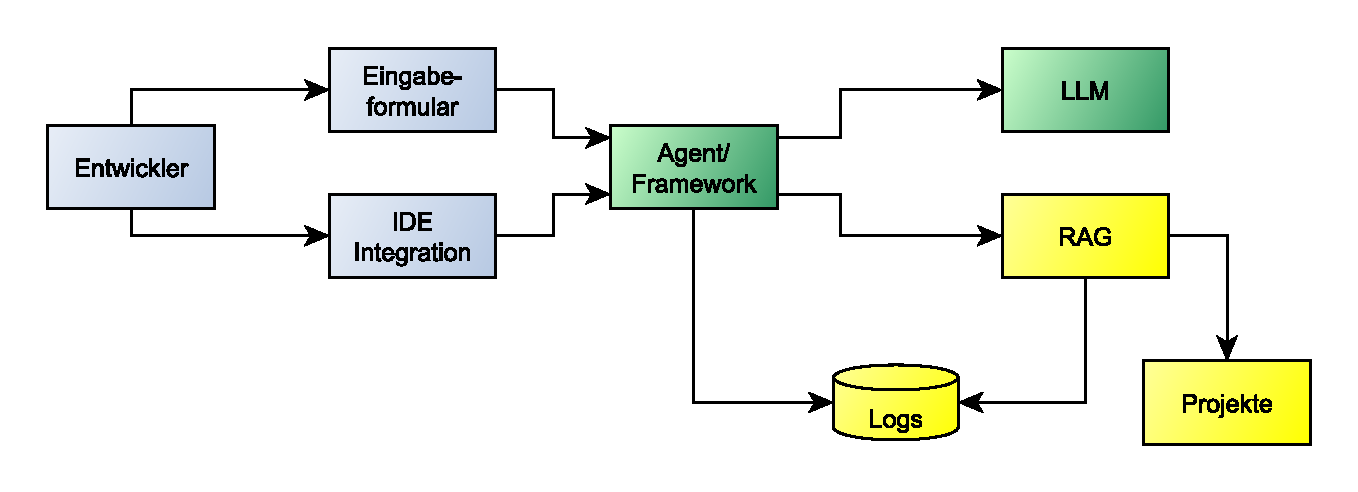
\includegraphics[width=0.9\textwidth]{content/chapter_discussion/images/anwendungsbeispiel.eps}
	\centering
	\caption{Anwendungsbeispiel für die Integration einer LLM}
	\label{img:example_firm_integration}
\end{figure}

Eine mögliche Erweiterung ist das Austauschen des Frameworks und der Einsatz eines Agenten. Im Weiteren kann ein \textit{Retrieval Augmented Generation} (\acrshort{RAG}) implementiert werden, um auf vorhandene firmenintern Daten zuzugreifen. Diese Daten können bereits gestellte Prompts der Entwickler oder vorhandener Code aus fertigen Projekten sein. Mit dem, in dieser Arbeit vorgestellten \texttt{DSPy} Framework können Agenten und RAG implementiert werden.\vspace{0.2cm}

Abschließend wird in Abbildung \ref{img:example_chat_form} ein Beispiel für ein einfaches Chat-Formular gezeigt. Weitere Formularfelder können im Formular hinzugefügt und der LLM als zusätzliche Metadaten oder Anweisungen mitgeteilt werden.\vspace{0.2cm}

\begin{figure}[!ht]
	
\includegraphics[width=0.8\textwidth]{content/chapter_discussion/images/chatbot_form_example.eps}
	\centering
	\caption{Anwendungsbeispiel für ein Eingabeformular für Prompts}
	\label{img:example_chat_form}
\end{figure}

%Blaupause für Prompting \href{https://piamedia.com/wp-content/uploads/2024/09/PIAM_Whitepaper_LLM-Halluzinationen_DE.pdf}{Das Geheimnis hinter LLM-Halluzinationen} [S. 16 ff.] noch testen und evaluieren.

%\href{https://arxiv.org/html/2501.16998v1}{Große Sprachmodelle zur Codegenerierung: Die Perspektive der Praktiker}

%Zur Optimierung des generierten Codes kann auch die freie Wahl der Softwarekomponenten durch die LLMs betragen. Wie in \cite{chen-2021} beschrieben können Nutzer, anstatt in Suchmaschinen beispielsweise die Vorteilen und Nachteile von \texttt{PyTorch} und \texttt{Tensorflow} zu vergleichen, kann das die LLM übernehmen und als Prompt wird nur \texttt{\# import machine learning package} angegeben.\vspace{0.2cm}

%Wie in [Quelle ist weg] beschrieben nimmt das Lesen von Programm zehn mal mehr Zeit in Anspruch, als Code zu schreiben. Diese Arbeit kann ebenfalls durch eine LLM übernommen werden.


\chapter{Fazit}\label{chap:conclusion}
\begin{tcolorbox}[
	enhanced,
	colback=red!5!white,
	colframe=red!75!black!50,
	title= Mein roter Faden
	]
	Struktur des Kapitels
	
	\begin{enumerate}
		\item \textbf{Zusammenfassung}: kurze Wiederholung der Zielsetzung d. Arbeit, Überblick der wichtigsten Ergebnisse aus Eval. und Optimierung, Fragestellung beantwortet?
		\item \textbf{Reflexion}: Stärken und Schwachen d. Arbeit, Diskussion über mögliche  Fehlerquellen, Einschätzung Optimierungsansätze oder Benchmarks
	\end{enumerate}
\end{tcolorbox}

\begin{tcolorbox}[
	enhanced,
	colback=red!5!white,
	colframe=red!75!black!50,
	title= Mein roter Faden
	]
	Unterschied Diskussion/Ausblick und Fazit\vspace{0.2cm}
	
	\begin{tabular}{|l|l|l|}
		\hline
		\textbf{Aspekt} & \textbf{Diskussion und Ausblick} & \textbf{Fazit} \\
		\hline
		\textbf{Funktion} & Kritische Analyse und & Zusammenfassung und \\
		& Zukunftsperspektive & Abschluss \\
		\hline
		\textbf{Zeitperspektive} & Zukunftsorientiert & Rückblickend \\
		\hline
		\textbf{Detaillierungsgrad} & Detailreichere Auseinandersetzung & Knapp und prägnant \\
		&  mit Ergebnissen & \\
		\hline
	\end{tabular}\vspace{0.2cm}
	
	Während \glqq Diskussion und Ausblick\grqq \ die Ergebnisse kritisch reflektiert und auf zukünftige Entwicklungen verweist, fasst das \glqq Fazit\grqq \ die Arbeit kompakt zusammen und beantwortet die Forschungsfrage. Beide Kapitel sind komplementär, aber klar voneinander zu unterscheiden.
\end{tcolorbox}

Es gibt Modelle welche besonders gut für die Webanwendungsentwicklung sehr gute Ergebnisse auch ohne Optimierung liefern. Dennoch sollte eine Optimierung in Betracht gezogen werden. Der Einsatz von generativer KI wird in alles Bereichen der Programmierung neue Maßstäbe setzen und nachhaltig verändern. Dieser Prozess hat bereits begonnen und mehr und mehr Unternehmen befassen sich mit diesem Thema. Dies bedeutet, dass eine Transformation der Prozesse für die Codegenerierung auf Unternehmensebene durchzuführen ist, auch wenn diese Transformation Kosten verursacht.\vspace{0.2cm}

Es kann aber festgestellt werden das ein einheitlicher Einsatz von optimierter generativer KI die Webanwendungsentwicklung effektiver gestalten wird, da auf Daten der zurückliegenden Projekte und Informationen aus den Interaktionen mit den LLMs zugegriffen werden kann. Des Weiteren kommt es dadurch langfristig zu einer Kosteneinsparung, da sich der Ressourcenverbrauch reduzieren wird. D.h. die Entwicklungszeit für Anwendungen wird reduziert, ebenso die Zeit bei der Fehlersuche und beim Implementieren von zusätzlichen Funktionen.
% Documents
% https://arxiv.org/abs/2109.04738: On the validity of pre-trained transformers for natural language processing in the software engineering domain
% https://arxiv.org/abs/2204.03214: Transformer-Based Language Models for Software Vulnerability Detection
%
% Tutorials
% https://towardsdatascience.com/building-a-python-code-generator-4b476eec5804